\documentclass[10pt]{article}
\usepackage[utf8]{inputenc}
\usepackage[T1]{fontenc}
\usepackage{amsmath}
\usepackage{amsfonts}
\usepackage{amssymb}
\usepackage[version=4]{mhchem}
\usepackage{stmaryrd}
\usepackage{mathrsfs}
\usepackage{graphicx}
\usepackage[export]{adjustbox}
\graphicspath{ {./images/} }
\usepackage{bbold}

\title{Neural Networks 
 Training, SGD and Backpropagation }

\author{}
\date{}


\begin{document}
\maketitle
Machine Learning Course - CS-433

Nov 7, 2023

Nicolas Flammarion

EPFL

\section*{Recap}
\section*{Neural Networks: Key Facts}
Supervised learning : we observe some data $S_{\text {train }}=\left\{x_{n}, y_{n}\right\}_{n=1}^{N} \in \mathscr{X} \times \mathscr{Y}$ $\Rightarrow$ given a new $x$, we want to predict its label $y$

Linear prediction (with augmented features): $\quad y=f_{\operatorname{Lin}}(x)=\phi(x)^{\top} w$ Features are given

Prediction with a NN:

$$
y=f_{\mathrm{NN}}(x)=f(x)^{\top} w
$$

\section*{Fully Connected Neural Networks}
Input
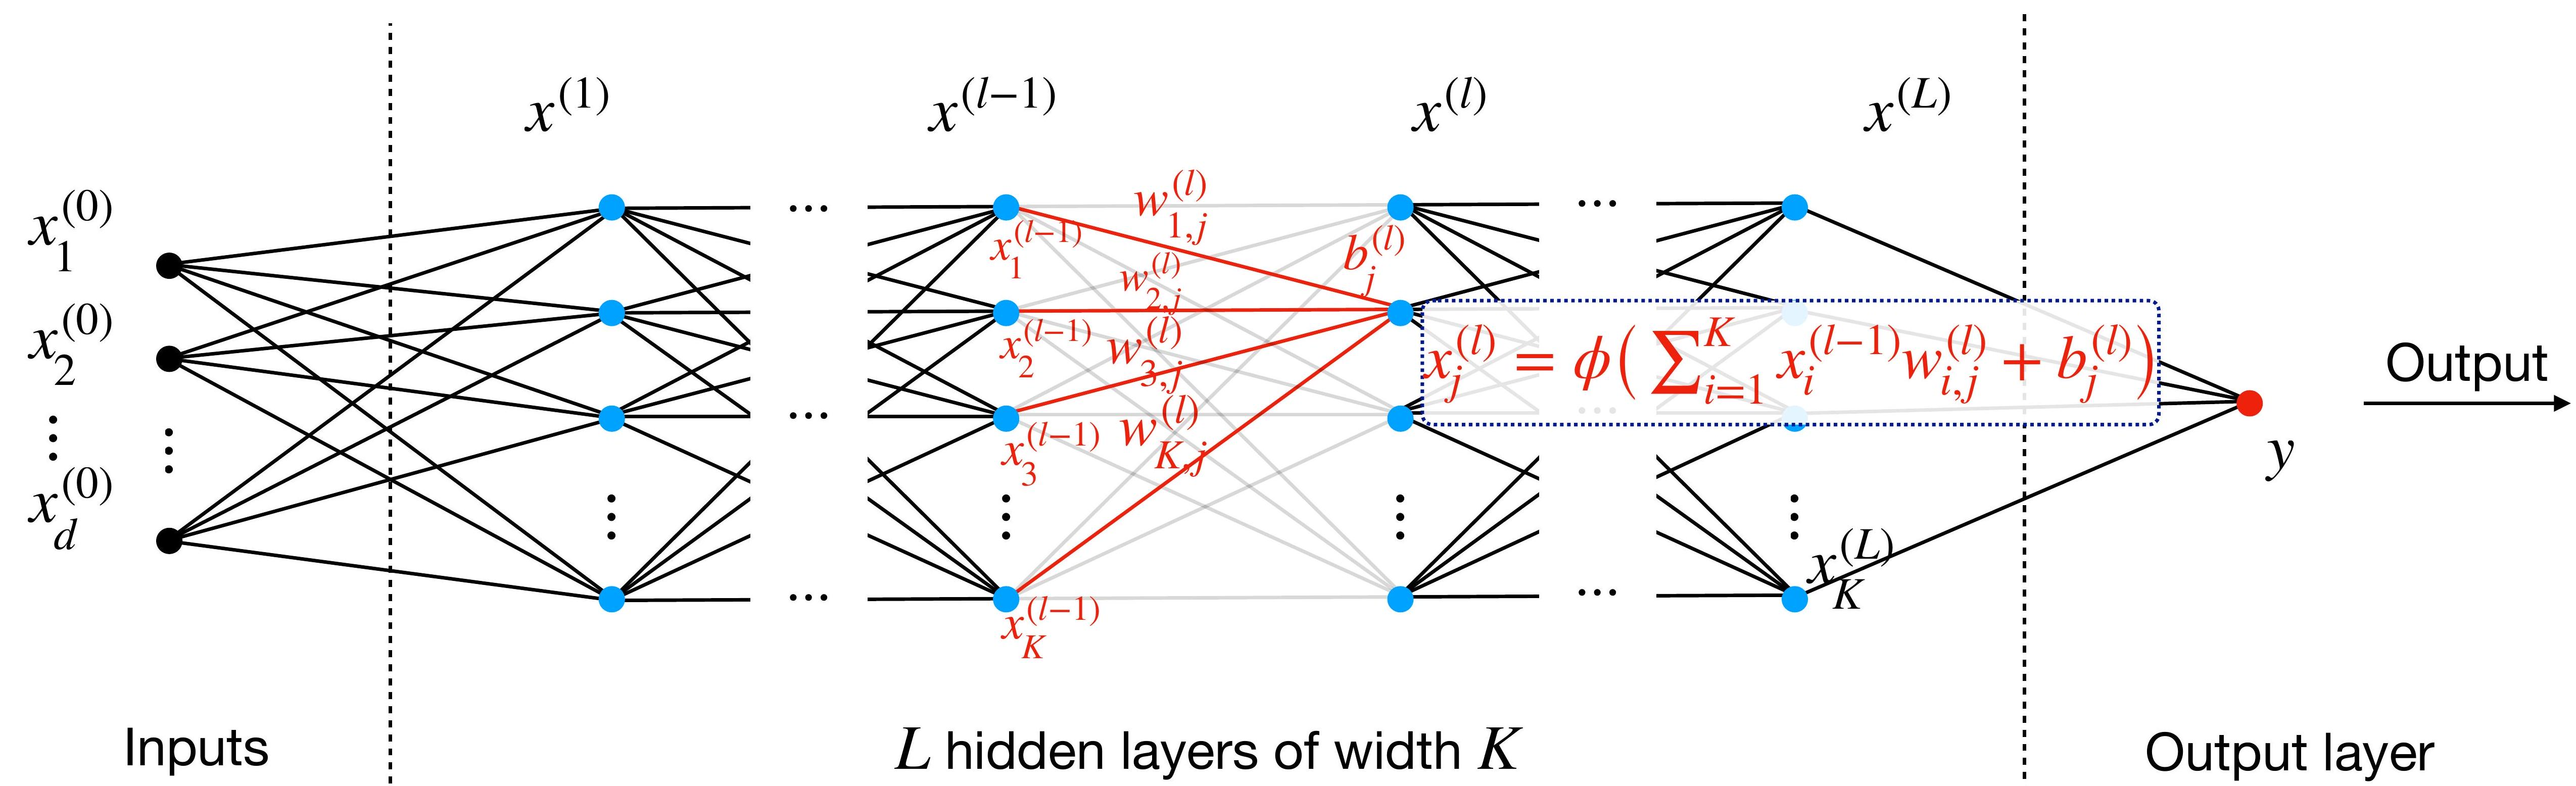
\includegraphics[max width=\textwidth, center]{2023_12_30_360102aa01a03e5a4270g-04}

$$
x_{j}^{(l)}=\phi\left(\sum_{i=1}^{K} x_{i}^{(l-1)} w_{i, j}^{(l)}+b_{j}^{(l)}\right)
$$

Important: $\phi$ is non-linear otherwise we can only represent linear functions

weight of the edge going from node $i$ in layer $l-1$ to node $j$ in layer $l$

bias term associated with node $j$ in layer $l$

\section*{NNs: Inference vs. Training}
Linear prediction on features $f(x)$

$$
h(x)=f(x)^{\top} w^{(L+1)}+b^{(L+1)}
$$

\begin{center}
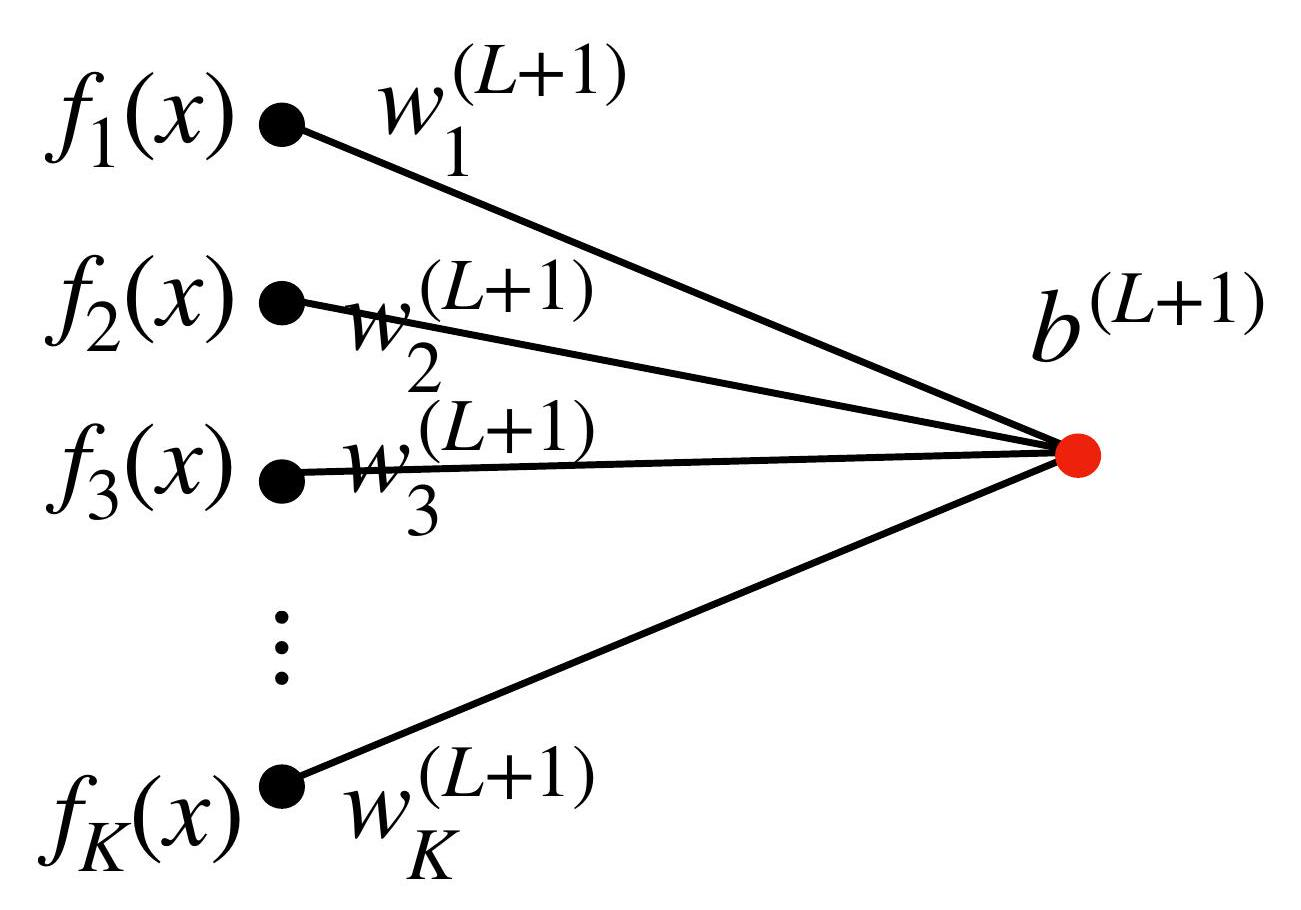
\includegraphics[max width=\textwidth]{2023_12_30_360102aa01a03e5a4270g-05}
\end{center}

Inference

$h(x)$

$\operatorname{sign}(h(x))$

Binary Classification

with $y \in\{-1,1\}$

Multi-Class Classification

with $y \in\{1, \ldots, K\}$

with $y \in \mathbb{R}$
Training

$\ell(y, h(x))=(h(x)-y)^{2}$

$\operatorname{argmax}_{c \in\{1, \ldots, K\}} h(x)_{c}$ $\ell(y, h(x))=\log (1+\exp (-y h(x)))$

$\ell(y, h(x))=-\log \frac{e^{h(x)_{y}}}{\sum_{i=1}^{K} e^{h(x)_{i}}}$

With a suitable representation of the data $f(x)$ learned by the network, the last layer only performs a linear regression or classification step

Today: How do we train a NN?

\section*{Training of NNs}
Training loss for a regression problem with $S_{\text {train }}=\left\{\left(x_{n}, y_{n}\right)\right\}_{n=1}^{N}$ :

$$
\mathscr{L}(f)=\frac{1}{2 N} \sum_{n=1}^{N}\left(y_{n}-f\left(x_{n}\right)\right)^{2}
$$

where $f$ is the function represented by a NN with weights $\left(w_{i, j}^{(l)}\right)$ and biases $\left(b_{i}^{(l)}\right)$

Task:

Remarks:

$$
\min _{w_{i, j}^{(l)}, b_{i}^{(l)}} \mathscr{L}(f)
$$

\begin{itemize}
  \item Regularization can be added to avoid overfitting and is easy to implement
  \item Non-convex optimization problem
\end{itemize}

$\Rightarrow$ not guaranteed to converge to a global minimum

\section*{Training of NNs with SGD}
SGD algorithm: Uniformly sample $n$, compute the gradient of $\mathscr{L}_{n}=\frac{1}{2}\left(y_{n}-f\left(x_{n}\right)\right)^{2}$ to update:

$$
\left(w_{i, j}^{(l)}\right)_{t+1}=\left(w_{i, j}^{(l)}\right)_{t}-\gamma \frac{\partial \mathscr{L}_{n}}{\partial w_{i, j}^{(l)}} \quad\left(b_{i}^{(l)}\right)_{t+1}=\left(b_{i}^{(l)}\right)_{t}-\gamma \frac{\partial \mathscr{L}_{n}}{\partial b_{i}^{(l)}}
$$

In Practice: Step size schedule, mini-batch, momentum, Adam

\section*{Training of NNs with SGD}
SGD algorithm: Uniformly sample $n$, compute the gradient of $\mathscr{L}_{n}=\frac{1}{2}\left(y_{n}-f\left(x_{n}\right)\right)^{2}$ to update:

$$
\left(w_{i, j}^{(l)}\right)_{t+1}=\left(w_{i, j}^{(l)}\right)_{t}-\gamma \frac{\partial \mathscr{L}_{n}}{\partial w_{i, j}^{(l)}} \quad\left(b_{i}^{(l)}\right)_{t+1}=\left(b_{i}^{(l)}\right)_{t}-\gamma \frac{\partial \mathscr{L}_{n}}{\partial b_{i}^{(l)}}
$$

In Practice: Step size schedule, mini-batch, momentum, Adam

Problem: With $O\left(K^{2} L\right)$ parameters, applying chain-rules independently is inefficient due to the compositional structure of $f$

Solution: the Backpropagation algorithm computes gradients via the chain rule but reuses intermediate computations

\section*{Description of NN parameters}
Input

\begin{center}
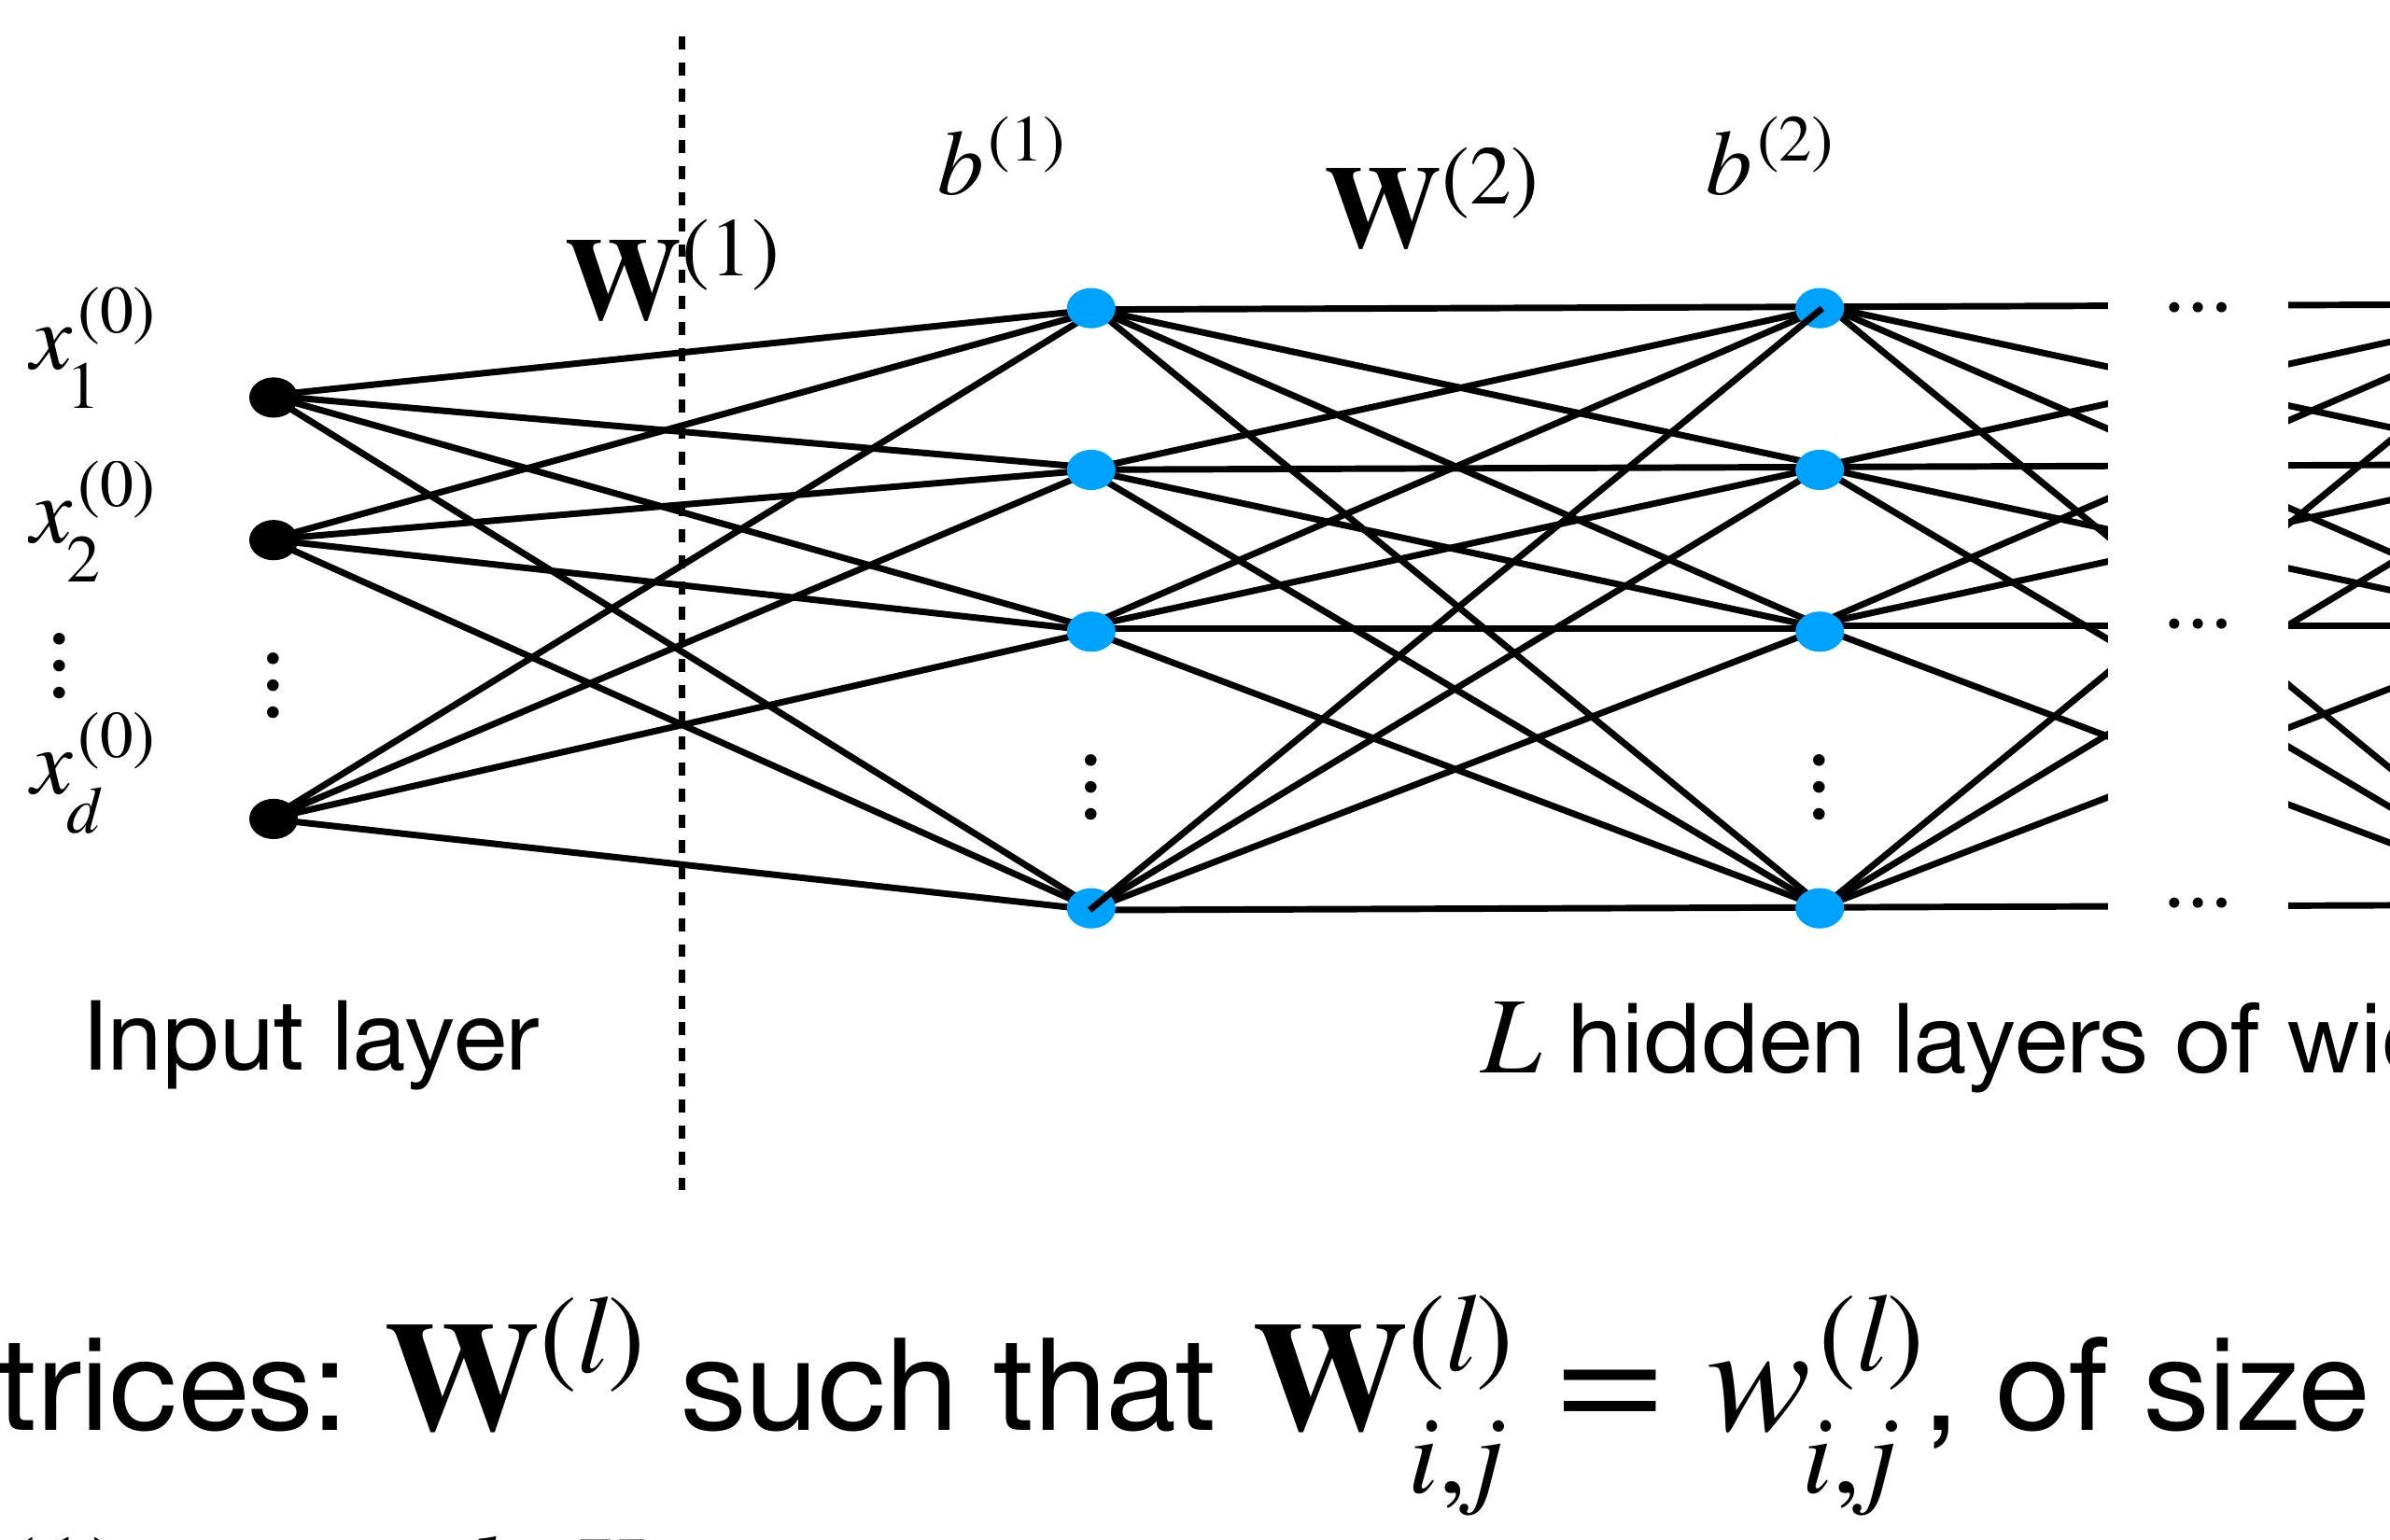
\includegraphics[max width=\textwidth]{2023_12_30_360102aa01a03e5a4270g-10(1)}
\end{center}

\begin{itemize}
  \item $\mathbf{W}^{(1)} \in \mathbb{R}^{d \times K}$
\end{itemize}

\begin{center}
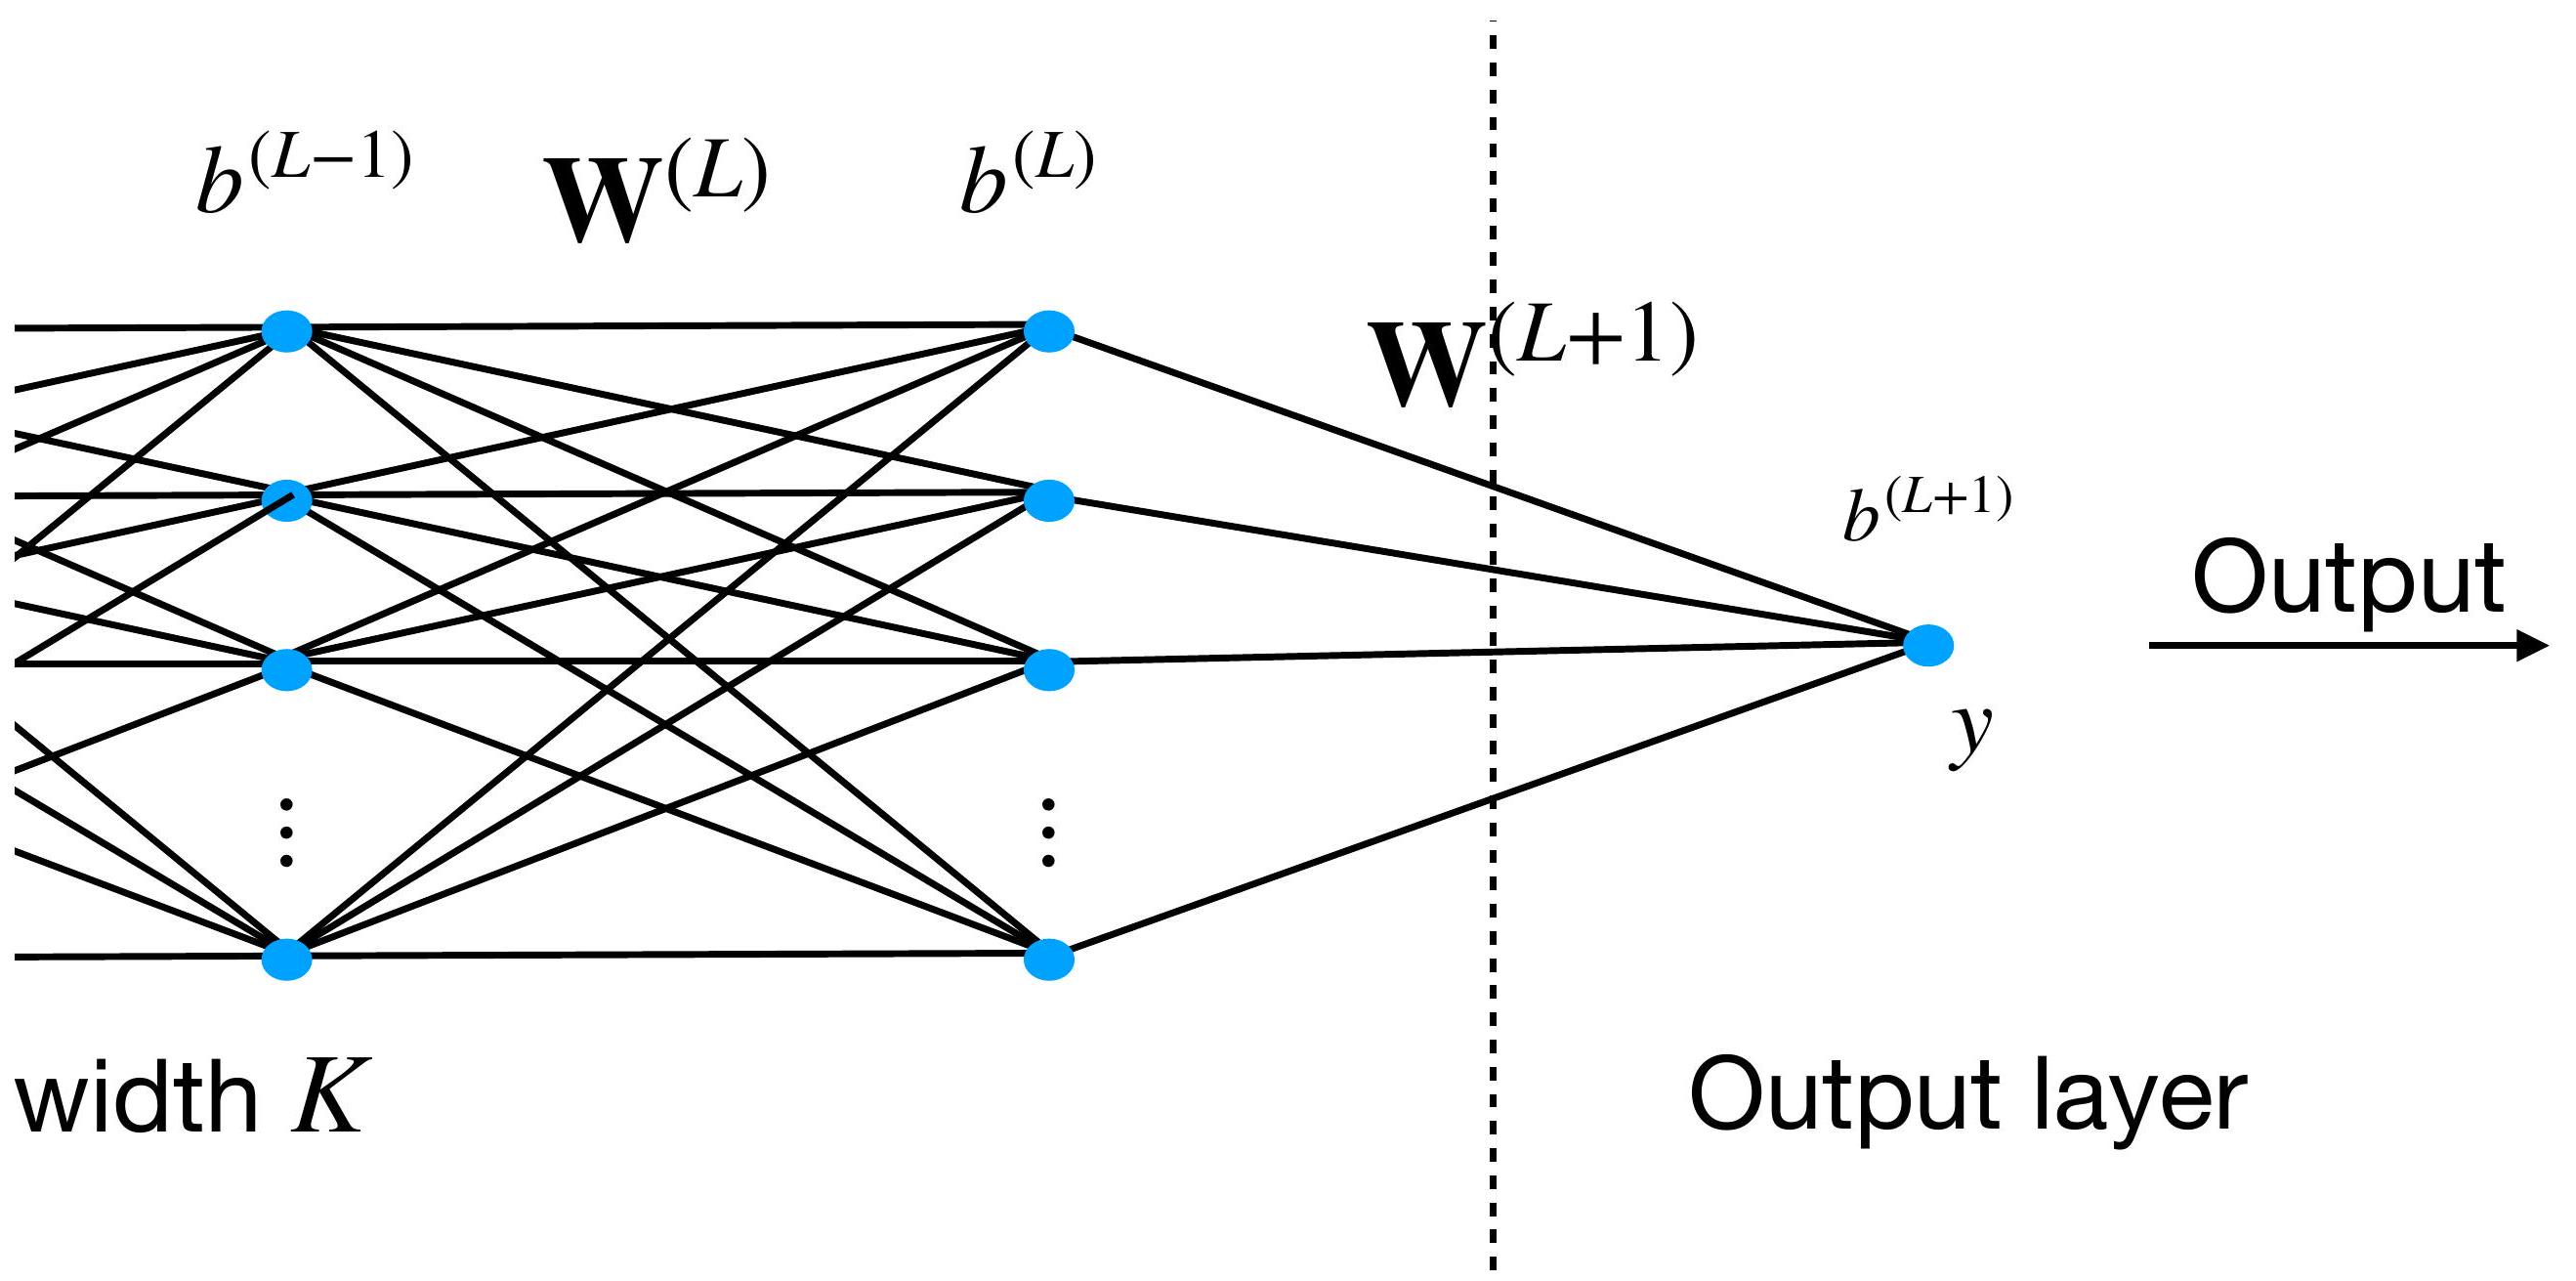
\includegraphics[max width=\textwidth]{2023_12_30_360102aa01a03e5a4270g-10}
\end{center}

Weight matrices: $\mathbf{W}^{(l)}$ such that $\mathbf{W}_{i, j}^{(l)}=w_{i, j}^{(l)}$, of size

\begin{itemize}
  \item $\mathbf{W}^{(l)} \in \mathbb{R}^{K \times K}$ for $2 \leq l \leq L$
  \item $\mathbf{W}^{(L+1)} \in \mathbb{R}^{K}$
\end{itemize}

Bias vectors: $b^{(l)}$ such that the i-th component is $b_{i}^{(l)}$

\begin{itemize}
  \item $b^{(l)} \in \mathbb{R}^{K}$ for $1 \leq l \leq L$
  \item $b^{(L+1)} \in \mathbb{R}$
\end{itemize}

\section*{Compact description of output}
The functions implemented by each layer can be written as:

\begin{itemize}
  \item $x^{(1)}=f^{(1)}\left(x^{(0)}\right):=\phi\left(\left(\mathbf{W}^{(1)}\right)^{\top} x^{(0)}+b^{(1)}\right)$
  \item $x^{(l)}=f^{(l)}\left(x^{(l-1)}\right):=\phi\left(\left(\mathbf{W}^{(l)}\right)^{\top} x^{(l-1)}+b^{(l)}\right)$
  \item $y=f^{(L+1)}\left(x^{(L)}\right):=\left(\mathbf{W}^{(L+1)}\right)^{\top} x^{(L)}+b^{(L+1)}$
\end{itemize}

The overall function $y=f\left(x^{(0)}\right)$ is just the composition of the layer functions:

$$
f=f^{(L+1)} \circ f^{(L)} \circ \cdots \circ f^{(l)} \circ \cdots \circ f^{(2)} \circ f^{(1)}
$$

\section*{Cost function}
Cost function:

$$
\mathscr{L}=\frac{1}{2 N} \sum_{n=1}^{N}\left(y_{n}-f^{(L+1)} \circ \cdots \circ f^{(2)} \circ f^{(1)}\left(x_{n}\right)\right)^{2}
$$

Remarks:

\begin{itemize}
  \item The specific form of the loss is not crucial
  \item $\mathscr{L}$ is a function of all weight matrices and bias vectors
  \item Each function $f^{(l)}$ is parameterized by weights $\mathbf{W}^{(l)}$ and biases $b^{(l)}$
\end{itemize}

Individual loss for SGD:

$$
\mathscr{L}_{n}=\frac{1}{2}\left(y_{n}-f^{(L+1)} \circ \cdots \circ f^{(2)} \circ f^{(1)}\left(x_{n}\right)\right)^{2}
$$

Goal: Compute for all $(i, j, l)$

$$
\frac{\partial \mathscr{L}_{n}}{\partial w_{i, j}^{(l)}} \quad \text { and } \quad \frac{\partial \mathscr{L}_{n}}{\partial b_{i}^{(l)}}
$$

\section*{Chain rule}
$$
\mathscr{L}_{n}=\frac{1}{2}\left(y_{n}-f^{(L+1)} \circ \cdots \circ f^{(l+1)} \circ \phi(\underbrace{\left.\left(\mathbf{W}^{(l)}\right)^{\top} x^{(l-1)}+b^{(l)}\right)}_{z^{(l)}})\right)^{2}
$$

\begin{center}
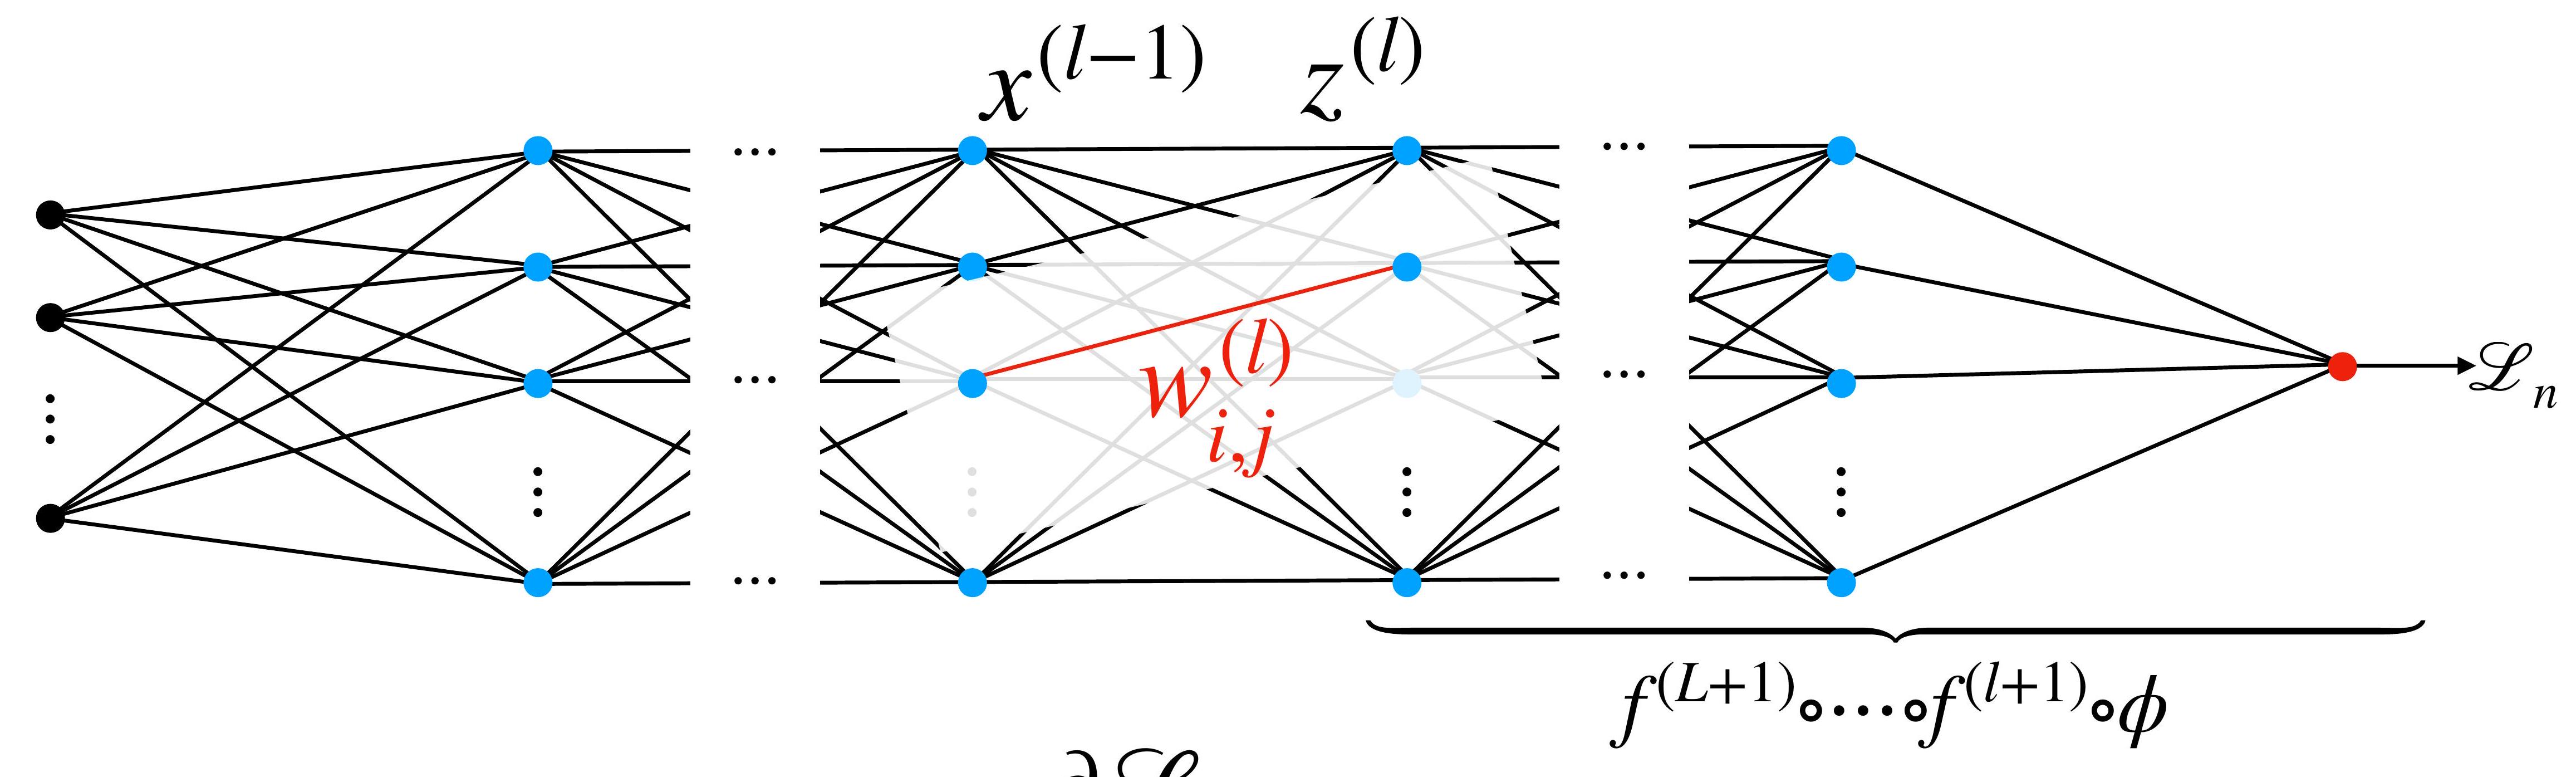
\includegraphics[max width=\textwidth]{2023_12_30_360102aa01a03e5a4270g-13}
\end{center}

$$
\frac{\partial \mathscr{L}_{n}}{\partial w_{i, j}^{(l)}} \quad ?
$$

\section*{Chain rule}
$$
\mathscr{L}_{n}=\frac{1}{2}\left(y_{n}-f^{(L+1)} \circ \cdots \circ f^{(l+1)} \circ \phi\left(z^{(l)}\right)\right)^{2}
$$

Apply the chain rule:
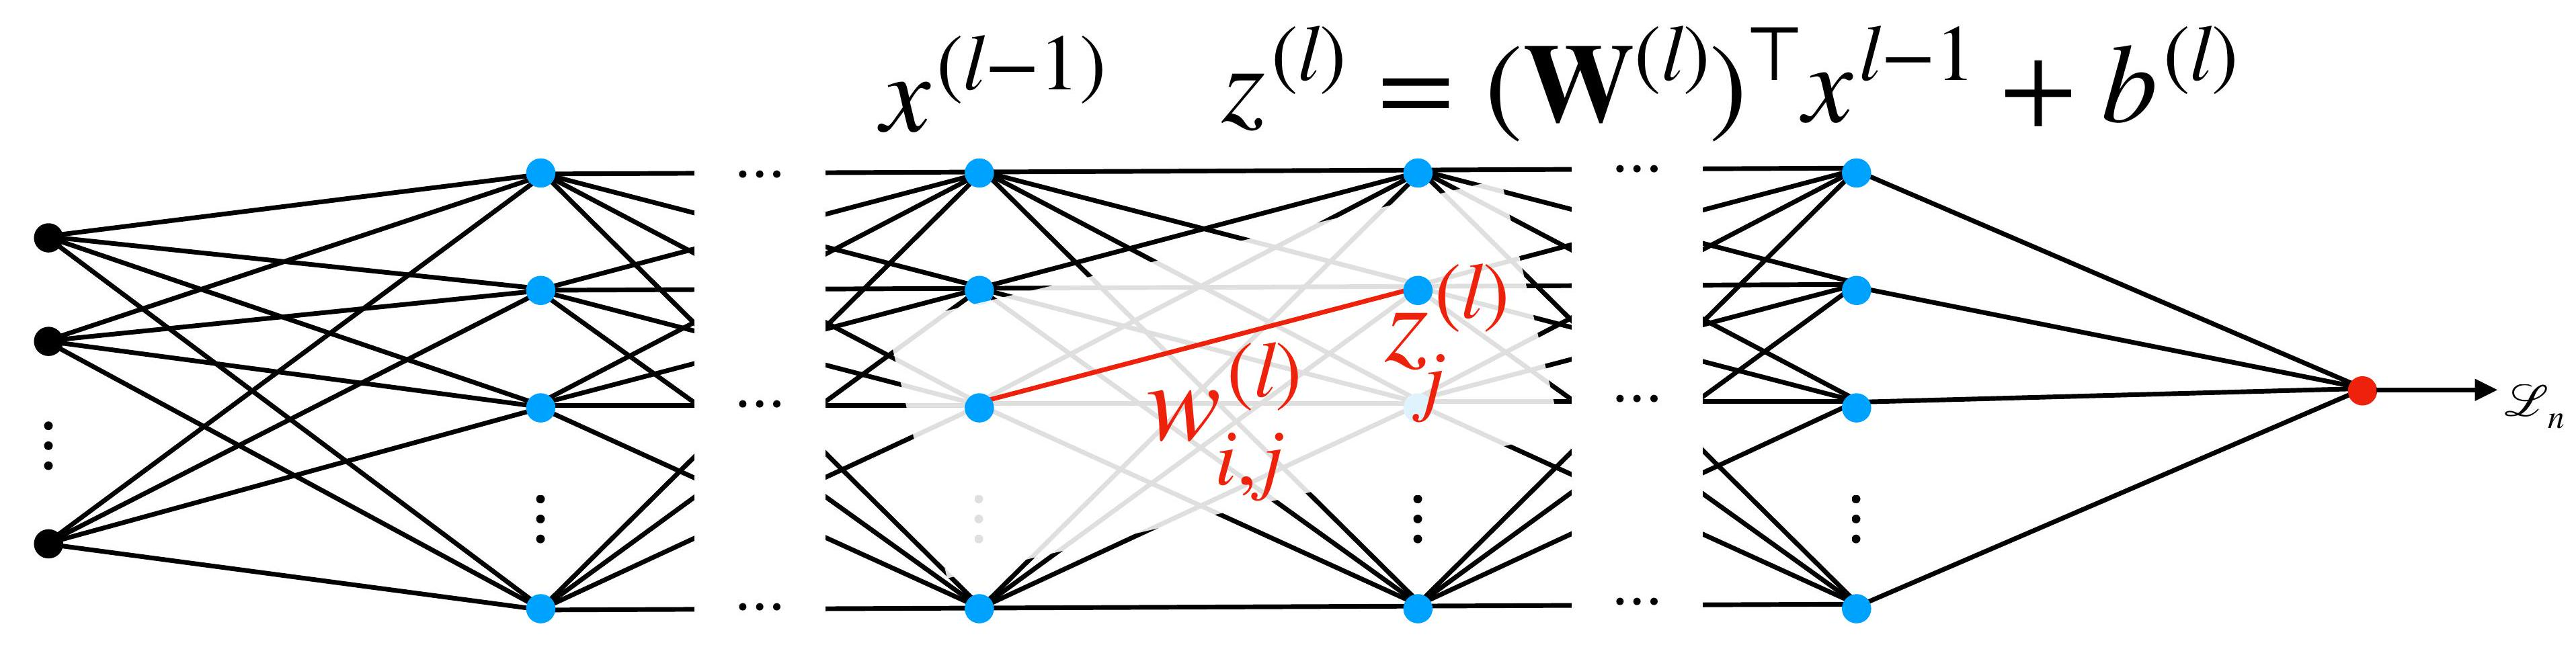
\includegraphics[max width=\textwidth, center]{2023_12_30_360102aa01a03e5a4270g-14}

$$
\begin{aligned}
\frac{\partial \mathscr{L}_{n}}{\partial w_{i, j}^{(l)}} & =\sum_{k=1}^{K} \frac{\partial \mathscr{L}_{n}}{\partial z_{k}^{(l)}} \frac{\partial z_{k}^{(l)}}{\partial w_{i, j}^{(l)}} \\
& =\frac{\partial \mathscr{L}_{n}}{\partial z_{j}^{(l)}} \frac{\partial z_{j}^{(l)}}{\partial w_{i, j}^{(l)}} \quad \text { since } \frac{\partial z_{k}^{(l)}}{\partial w_{i, j}^{(l)}}=0 \text { for } k \neq j \\
& =\frac{\partial \mathscr{L}_{n}}{\partial z_{j}^{(l)}} \cdot x_{i}^{(l-1)} \quad \text { since } z_{j}^{(l)}=\sum_{k=1}^{K} w_{k, j}^{(l)} x_{k}^{(l-1)}+b_{j}^{(l)}
\end{aligned}
$$

We need to compute $\frac{\partial \mathscr{L}_{n}}{\partial z_{j}^{(l)}}, z^{(l)}, x_{i}^{(l-1)}$ and reuse them for different $\frac{\partial \mathscr{L}_{n}}{\partial w_{i, j}^{(l)}}$

\section*{Forward Pass}
We can compute $z^{(l)}$ and $x^{(l)}$ by a forward pass in the network:

$$
\begin{aligned}
& x^{(0)}=x_{n} \in \mathbb{R}^{d} \\
& z^{(l)}=\left(\mathbf{W}^{(l)}\right)^{\top} x^{(l-1)}+b^{(l)} \\
& x^{(l)}=\phi\left(z^{(l)}\right)
\end{aligned}
$$

Computational complexity:

\begin{center}
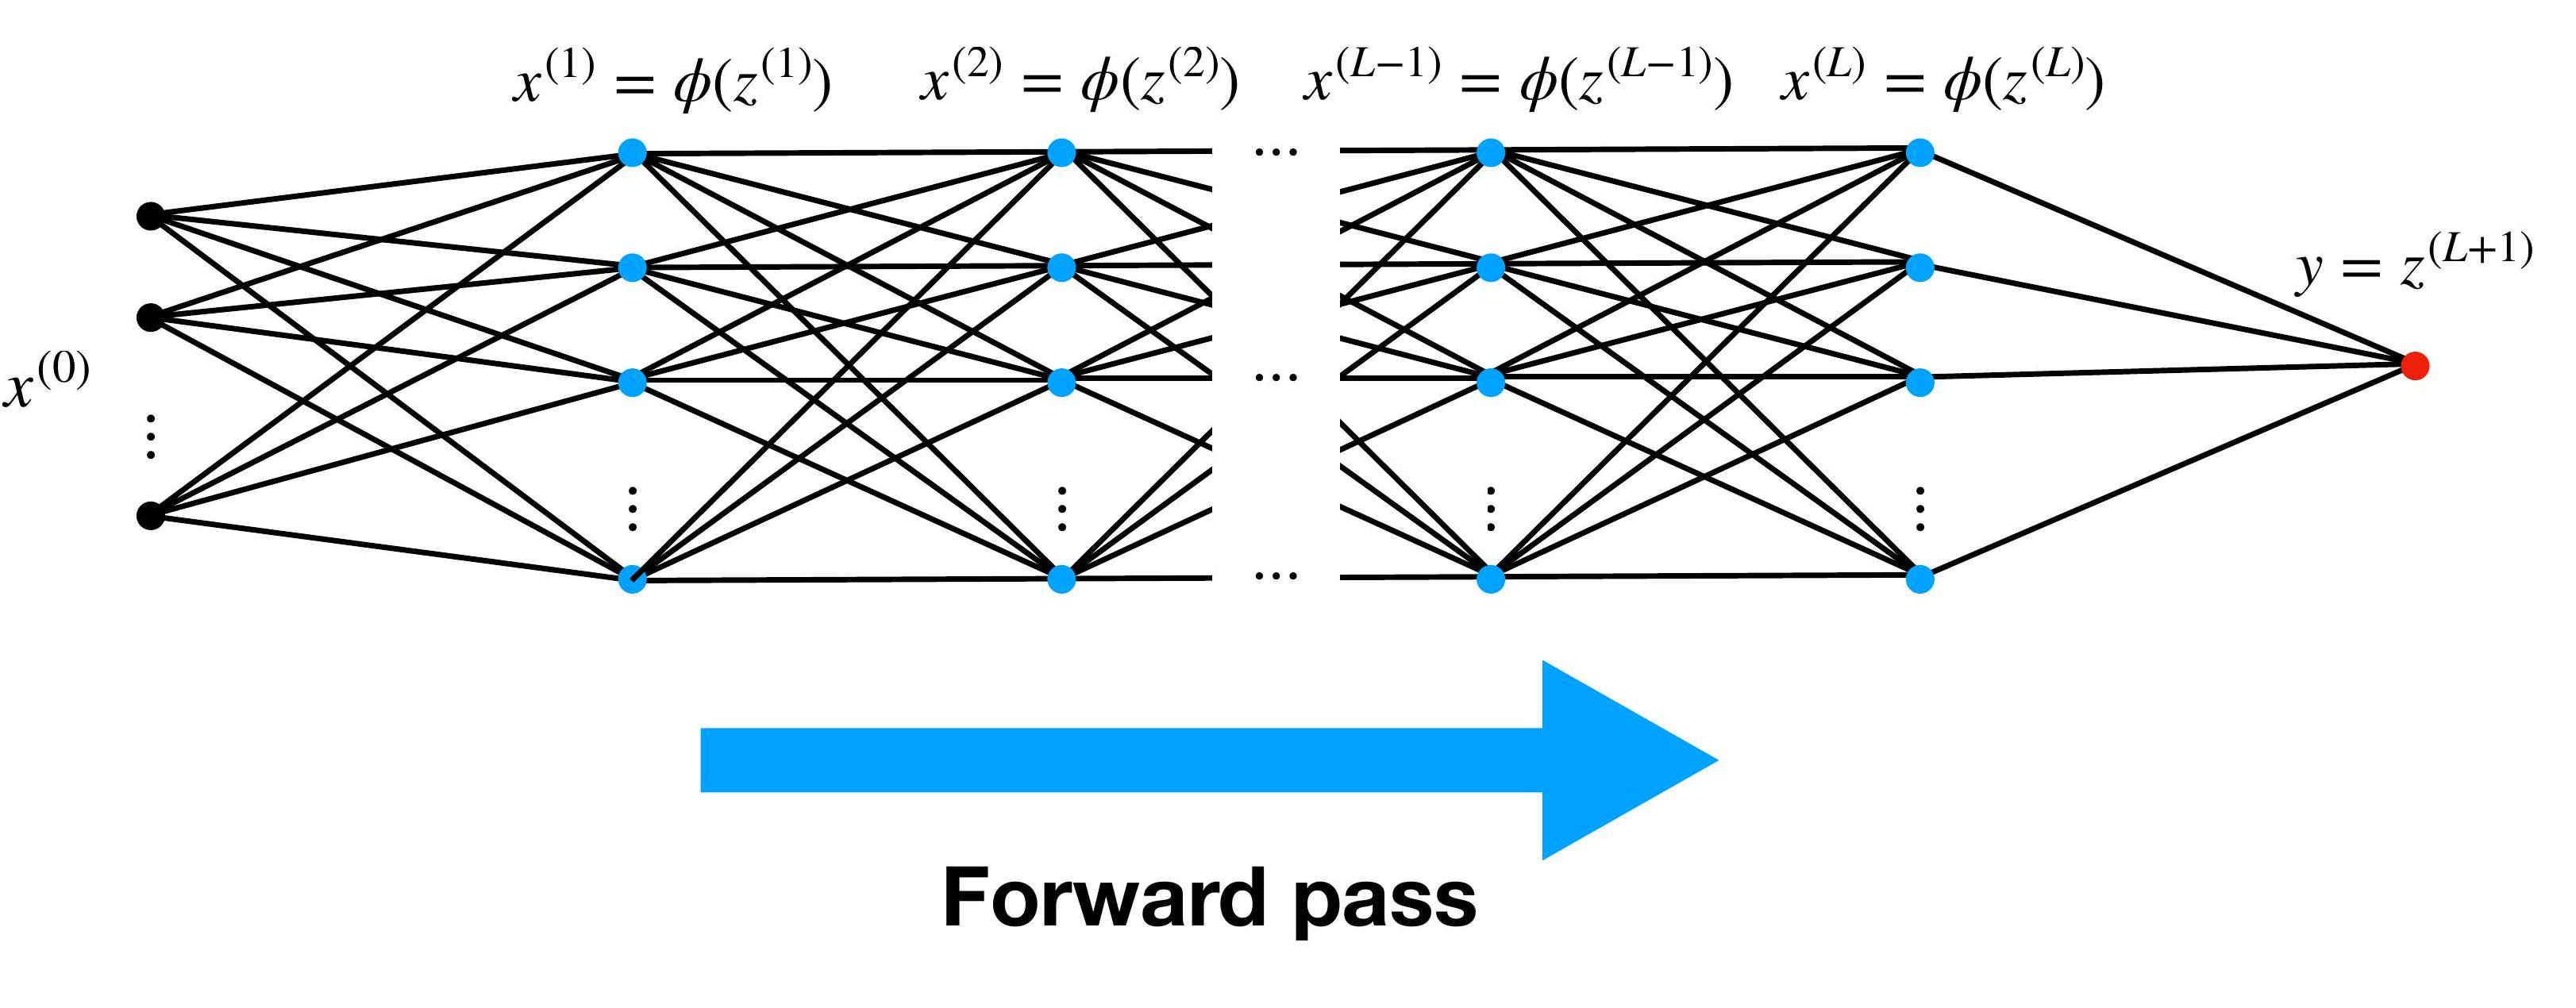
\includegraphics[max width=\textwidth]{2023_12_30_360102aa01a03e5a4270g-15}
\end{center}

$\Rightarrow$ one pass over the network $O\left(K^{2} L\right)$

\section*{Backward pass (I)}
Define $\delta_{j}^{(l)}=\frac{\partial \mathscr{L}_{n}}{\partial z_{j}^{(l)}}$
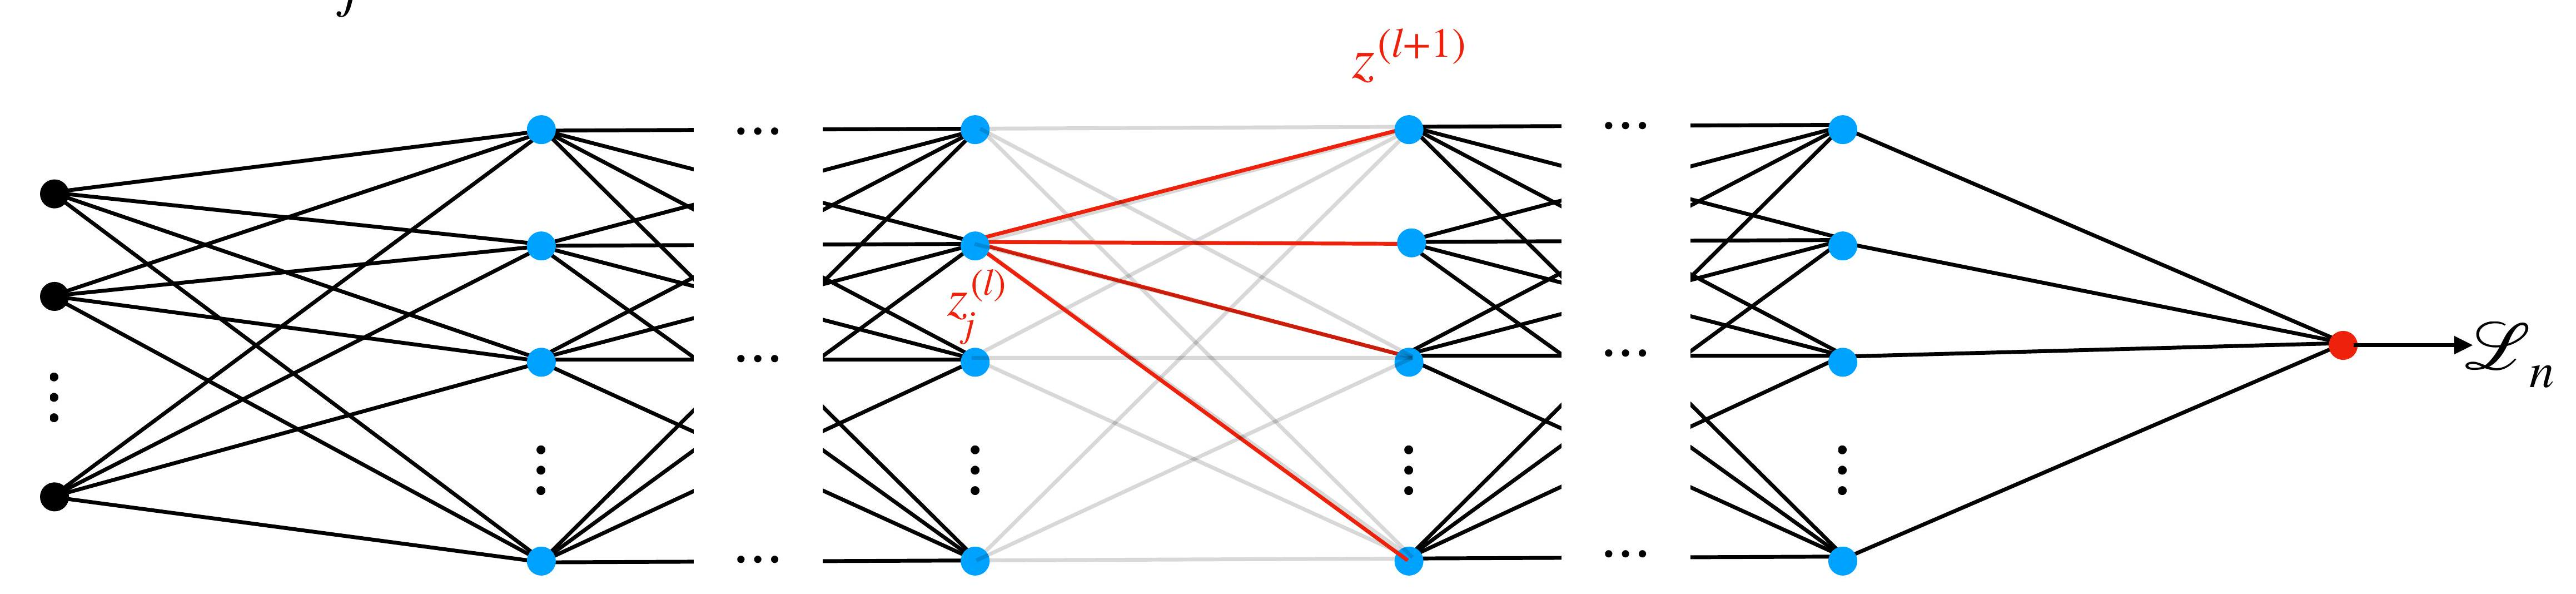
\includegraphics[max width=\textwidth, center]{2023_12_30_360102aa01a03e5a4270g-16}

Chain rule:

$$
\delta_{j}^{(l)}=\frac{\partial \mathscr{L}_{n}}{\partial z_{j}^{(l)}}=\sum_{k} \frac{\partial \mathscr{L}_{n}}{\partial z_{k}^{(l+1)}} \frac{\partial z_{k}^{(l+1)}}{\partial z_{j}^{(l)}}=\sum_{k} \delta_{k}^{(l+1)} \frac{\partial z_{k}^{(l+1)}}{\partial z_{j}^{(l)}}
$$

\section*{Backward pass (II)}
Using $z_{k}^{(l+1)}=\sum_{i=1}^{K} w_{i, k}^{(l+1)} x_{i}^{(l)}+b_{k}^{(l+1)}=\sum_{i=1}^{K} w_{i, k}^{(l+1)} \phi\left(z_{i}^{(l)}\right)+b_{k}^{(l+1)}$

We obtain $\frac{\partial z_{k}^{(l+1)}}{\partial z_{j}^{(l)}}=\phi^{\prime}\left(z_{j}^{(l)}\right) w_{j, k}^{(l+1)}$

Thus

$$
\delta_{j}^{(l)}=\sum_{k} \delta_{k}^{(l+1)} \phi^{\prime}\left(z_{j}^{(l)}\right) w_{j, k}^{(l+1)}
$$

It can be written in vector form:

$$
\delta^{(l)}=\left(\mathbf{W}^{(l+1)} \delta^{(l+1)}\right) \odot \phi^{\prime}\left(z^{(l)}\right)
$$

\section*{Backward pass (III)}
Initialization:

$$
\begin{aligned}
\delta^{(L+1)} & =\frac{\partial}{\partial z^{(L+1)}} \frac{1}{2}\left(y_{n}-z^{(L+1)}\right)^{2} \\
& =z^{(L+1)}-y_{n}
\end{aligned}
$$

\begin{center}
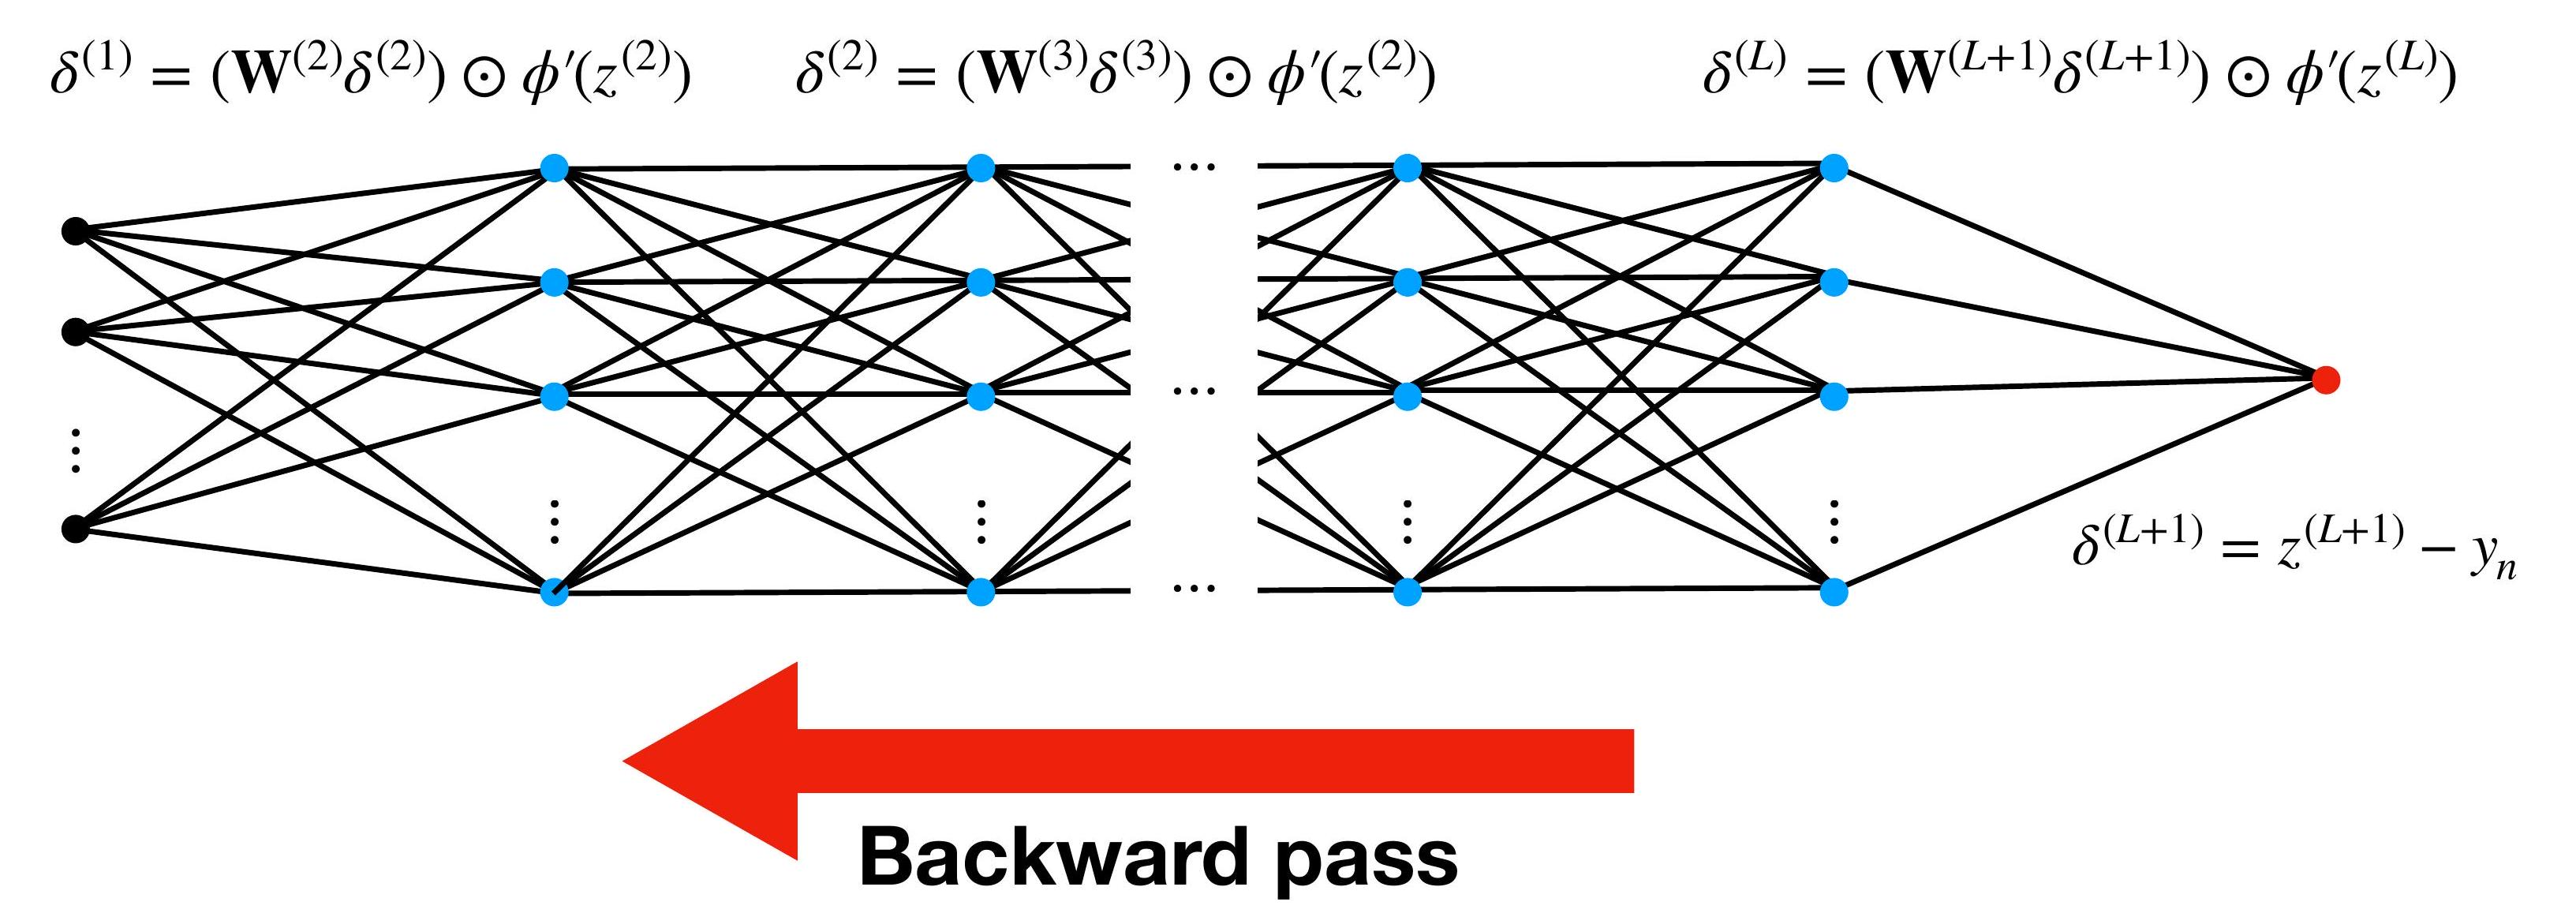
\includegraphics[max width=\textwidth]{2023_12_30_360102aa01a03e5a4270g-18}
\end{center}

Compute all the $\delta^{(l)}$ by a backward pass in the network:

$$
\delta^{(l)}=\left(\mathbf{W}^{(l+1)} \delta^{(l+1)}\right) \odot \phi^{\prime}\left(z^{(l)}\right)
$$

Computational complexity: one pass over the network $O\left(K^{2} L\right)$

\section*{Derivatives computation}
\begin{center}
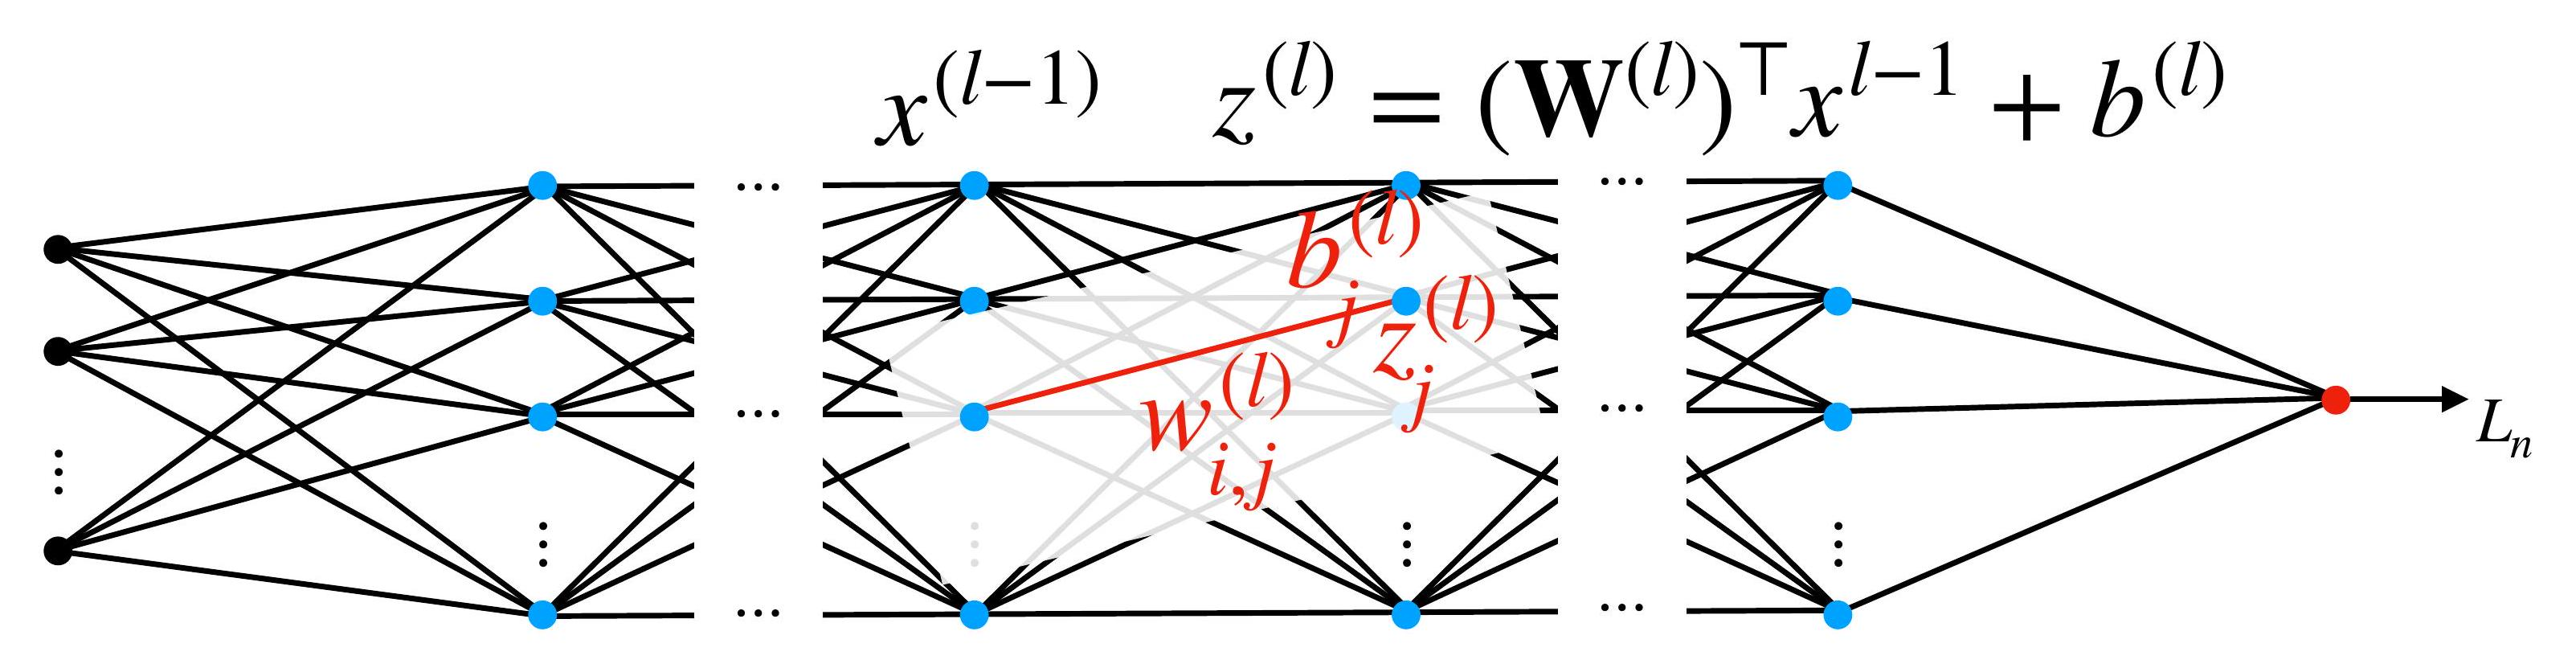
\includegraphics[max width=\textwidth]{2023_12_30_360102aa01a03e5a4270g-19}
\end{center}

Using that $z_{m}^{(l)}=\sum_{k=1}^{K} w_{k, m}^{(l)} x_{k}^{(l-1)}+b_{m}^{(l)}$ :

\begin{itemize}
  \item $\frac{\partial \mathscr{L}_{n}}{\partial b_{j}^{(l)}}=\sum_{k=1}^{K} \frac{\partial \mathscr{L}_{n}}{\partial z_{k}^{(l)}} \frac{\partial z_{k}^{(l)}}{\partial b_{j}^{(l)}}=\frac{\partial \mathscr{L}_{n}}{\partial z_{j}^{(l)}} \frac{\partial z_{j}^{(l)}}{\partial b_{j}^{(l)}}=\delta_{j}^{(l)}$

  \item $\frac{\partial \mathscr{L}_{n}}{\partial w_{i, j}^{(l)}}=\sum_{k=1}^{K} \frac{\partial \mathscr{L}_{n}}{\partial z_{k}^{(l)}} \frac{\partial z_{k}^{(l)}}{\partial w_{i, j}^{(l)}}=\frac{\partial \mathscr{L}_{n}}{\partial z_{j}^{(l)}} \frac{\partial z_{j}^{(l)}}{\partial w_{i, j}^{(l)}}=\delta_{j}^{(l)} \cdot x_{i}^{(l-1)}$

\end{itemize}

\section*{Backpropagation algorithm}
Forward pass:

$$
\begin{aligned}
& x^{(0)}=x_{n} \in \mathbb{R}^{d} \\
& z^{(l)}=\left(\mathbf{W}^{(l)}\right)^{\top} x^{(l-1)}+b^{(l)} \\
& x^{(l)}=\phi\left(z^{(l)}\right)
\end{aligned}
$$

Backward pass:

$$
\begin{aligned}
& \delta^{(L+1)}=z^{(L+1)}-y_{n} \\
& \delta^{(l)}=\left(\mathbf{W}^{(l+1)} \delta^{(l+1)}\right) \odot \phi^{\prime}\left(z^{(l)}\right)
\end{aligned}
$$

\begin{center}
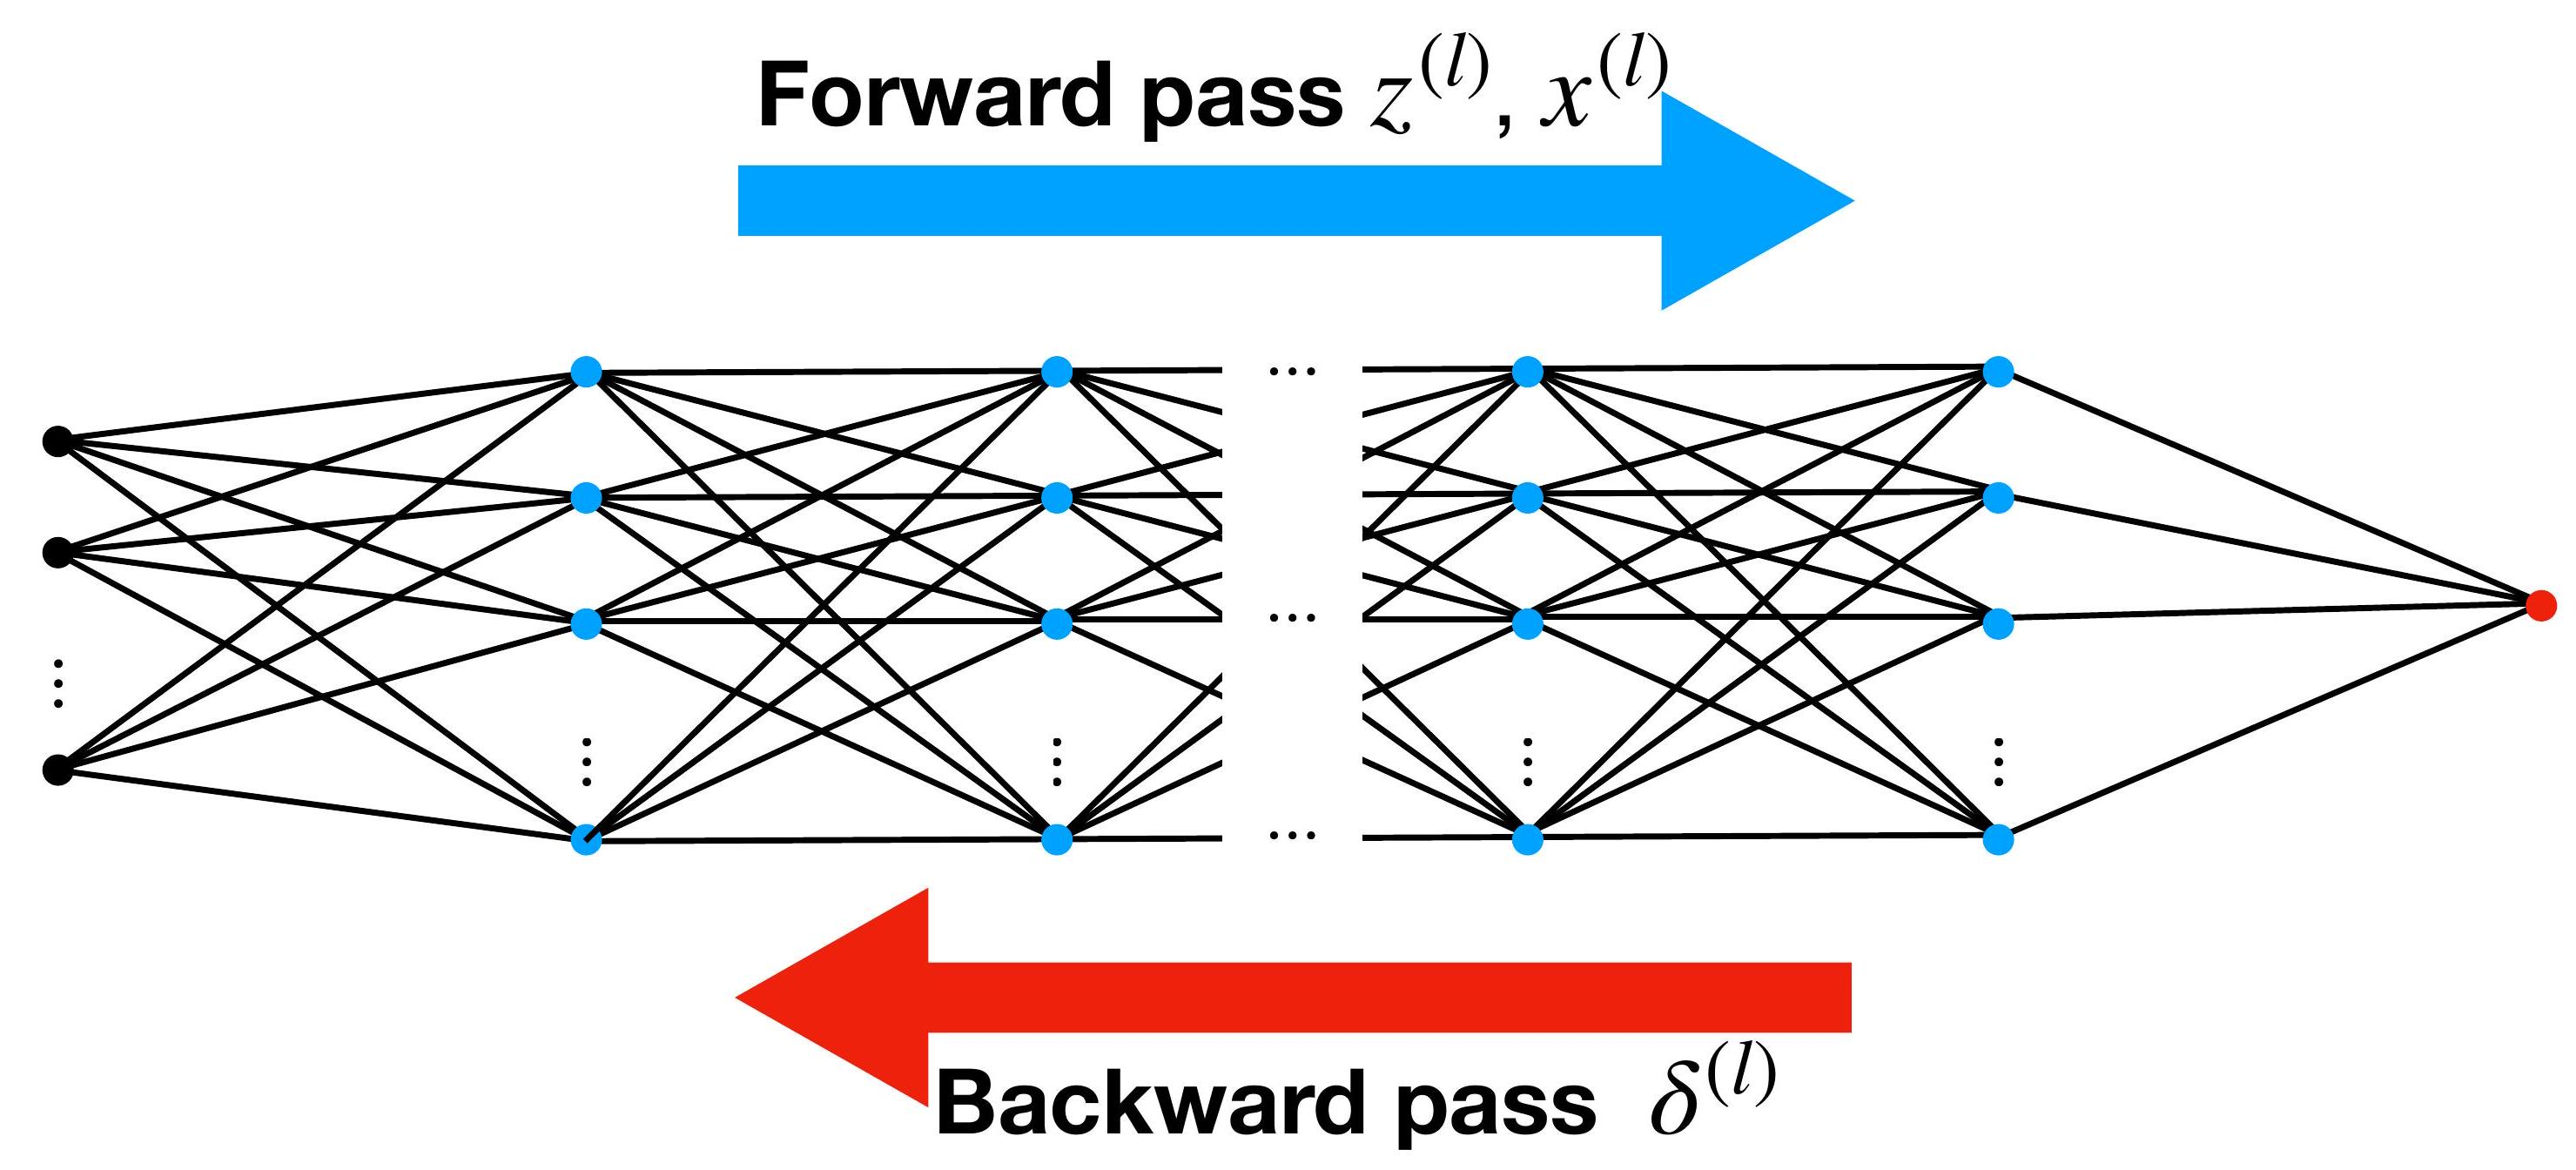
\includegraphics[max width=\textwidth]{2023_12_30_360102aa01a03e5a4270g-20}
\end{center}

Compute the derivatives:

$$
\begin{aligned}
& \frac{\partial \mathscr{L}_{n}}{\partial w_{i, j}^{(l)}}=\delta_{j}^{(l)} x_{i}^{(l-1)} \\
& \frac{\partial \mathscr{L}_{n}}{\partial b_{j}^{(l)}}=\delta_{j}^{(l)}
\end{aligned}
$$

\section*{Parameter Initialization}
\section*{Importance of Parameter Initialization}
\begin{itemize}
  \item In deep networks, improper parameter initialization can lead to the vanishing or exploding gradients problem

  \item Problem: Extremely slow or unstable optimization

  \item Solution: Control the layerwise variance of neurons (aka He initialization)

  \item Note: As illustrated, even a two-fold difference in the scale of

\end{itemize}

\begin{center}
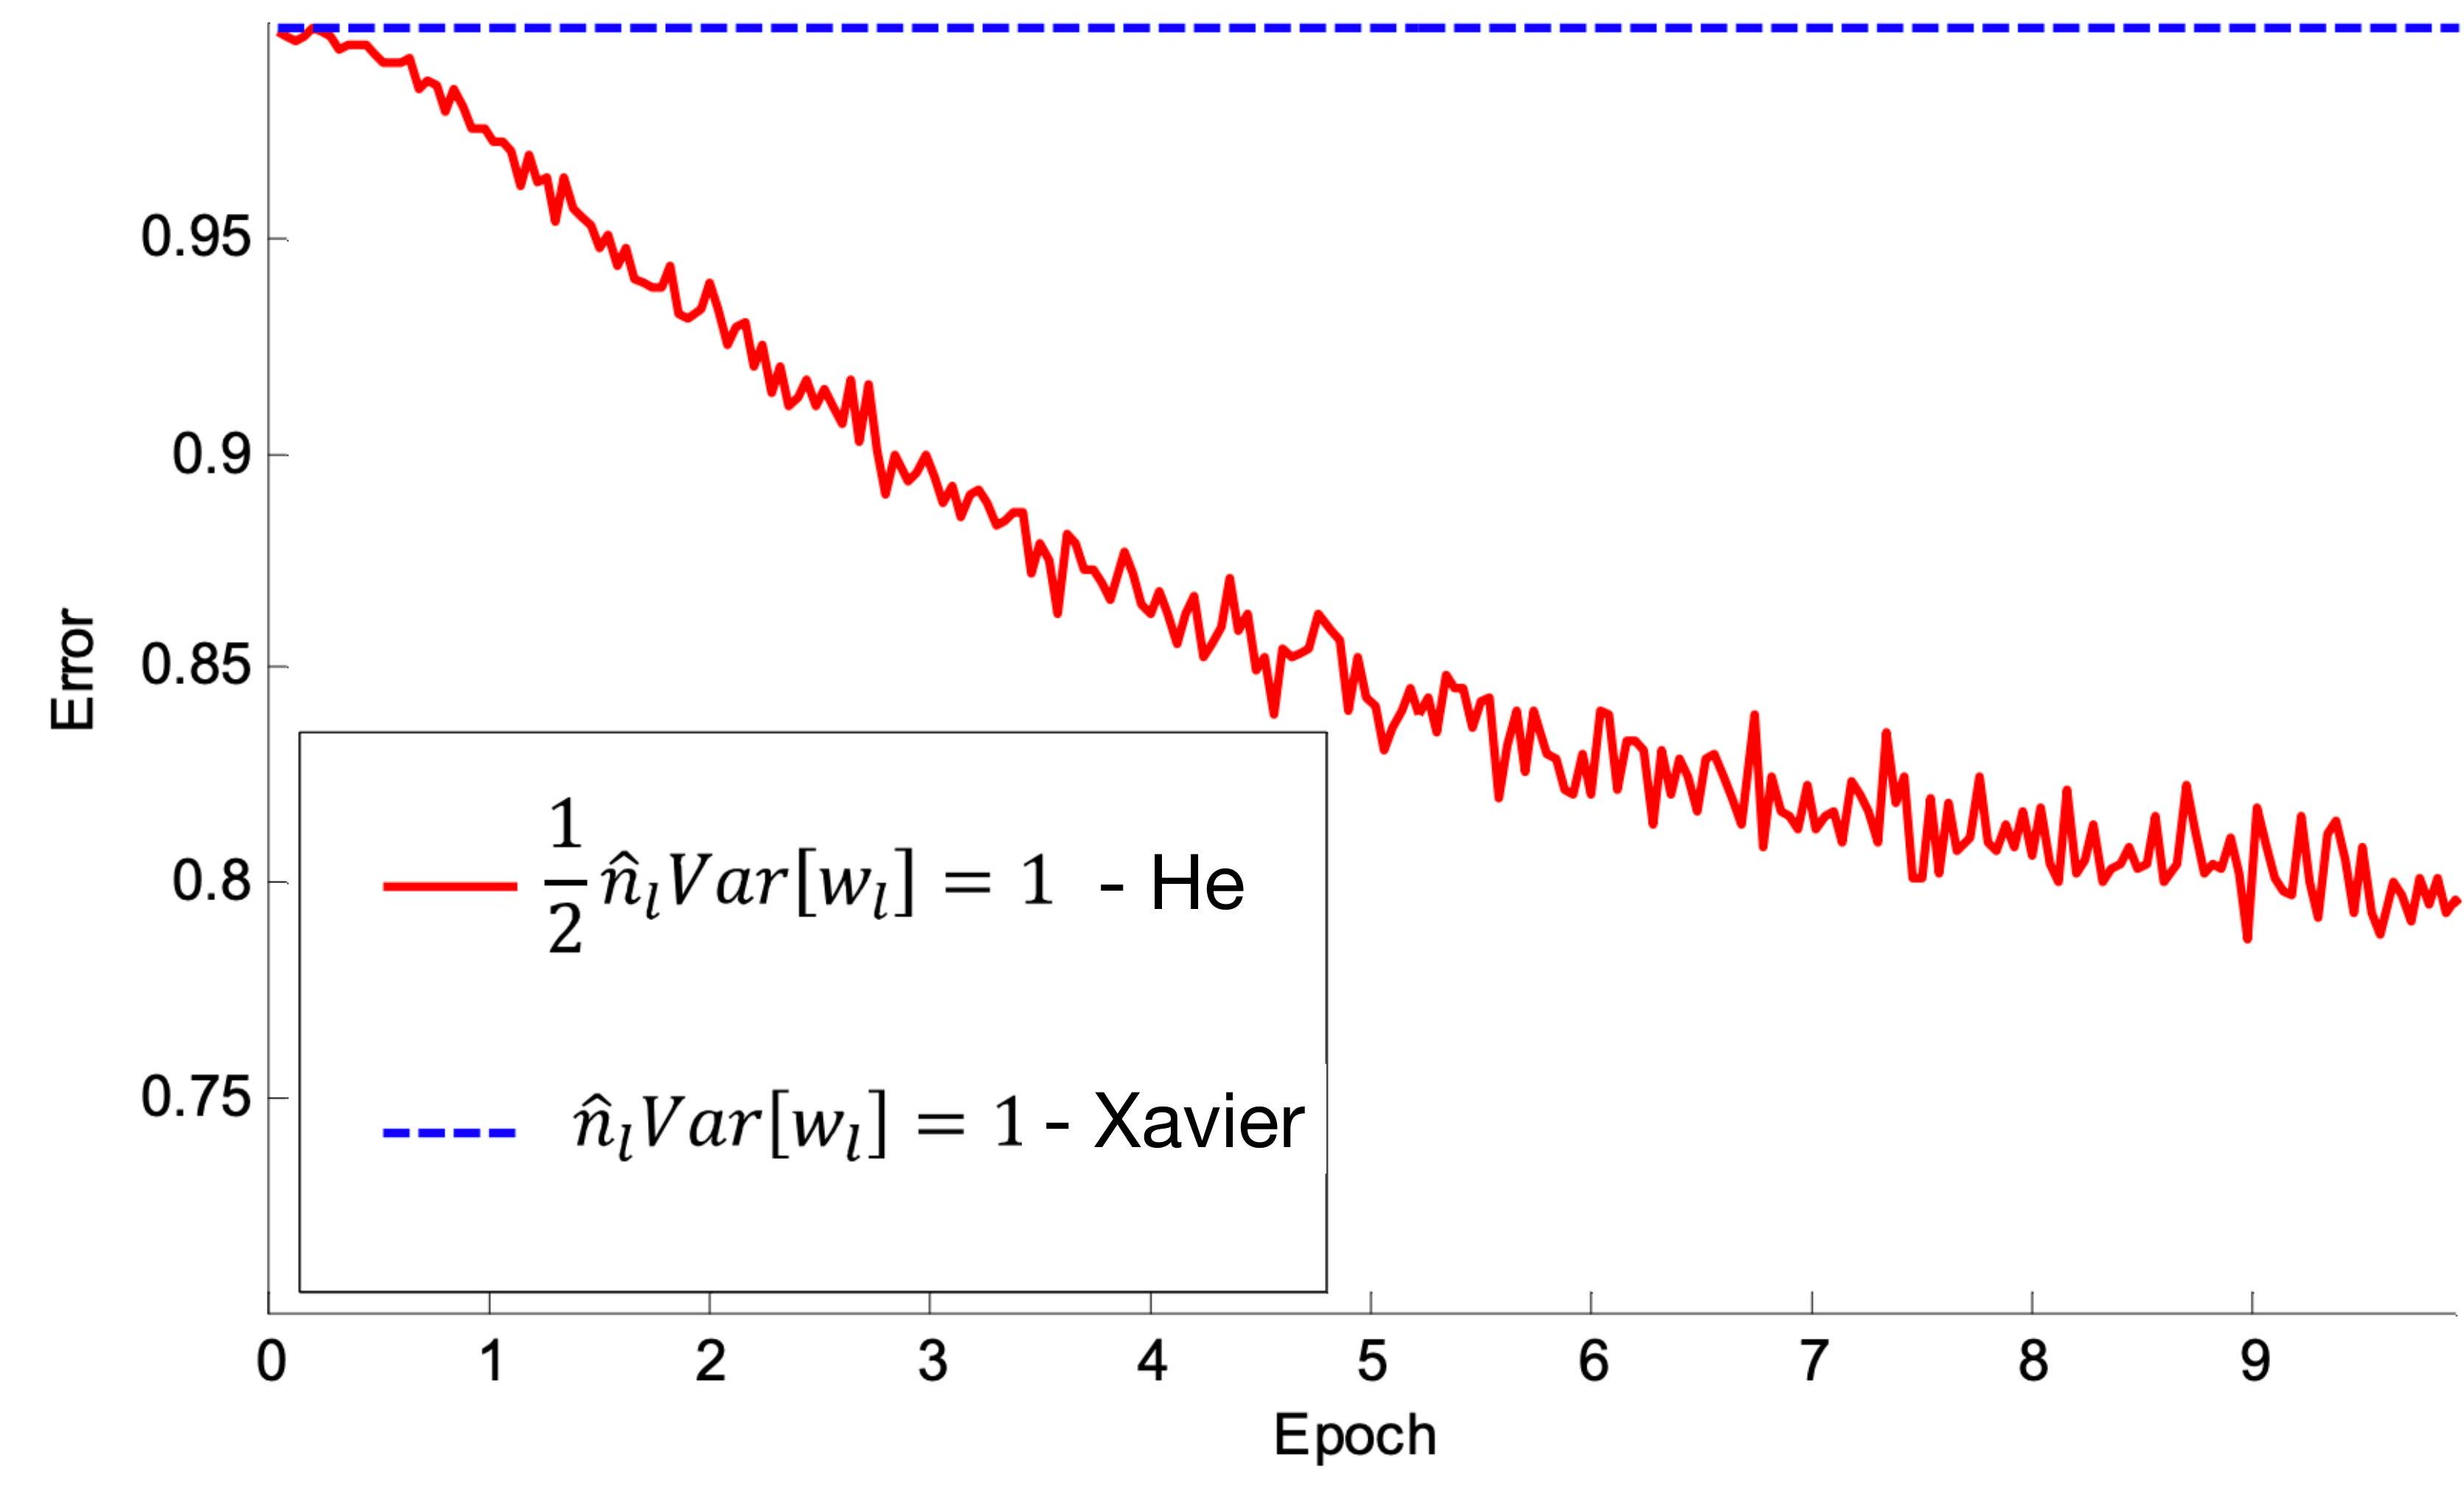
\includegraphics[max width=\textwidth]{2023_12_30_360102aa01a03e5a4270g-22}
\end{center}

Source: Delving Deep into Rectifiers: Surpassing Human-Level

Performance on ImageNet Classification (CVPR 2015) initialization can be crucial

\section*{Variance-Preserving Initialization}
Variance-preserving initialization for ReLU networks:

\begin{itemize}
  \item $z^{(l)} \sim \mathcal{N}\left(0, \mathbf{I}_{K}\right)$ : pre-activations at layer $l$ (note: $\operatorname{Var}\left[z_{i}^{(l)}\right]=1$ )

  \item $w_{i}^{(l+1)} \sim \mathcal{N}\left(0, \sigma \mathbf{I}_{K}\right)$ : the $i$-th weight vector at layer $l+1$

  \item $z_{i}^{(l+1)}=\operatorname{ReLU}\left(z^{(l)}\right)^{\top} w_{i}^{(l+1)}:$ the $i$-th pre-activation at layer $l+1$

\end{itemize}

Question: How should we set $\sigma$ so that $\operatorname{Var}\left[z_{i}^{(l+1)}\right]=1$ ?

Answer: $\sigma=\sqrt{2 / K}$

Derivation: Refer to the exercise for the derivation

\section*{Normalization Layers}
\section*{Batch Normalization}
Consider a batch $B=\left(x_{1}, \cdots, x_{M}\right)$ and denote by $z_{n}^{(l)}$ the layer's pre-activation input corresponding to the observation $x_{n}$

\section*{Batch Normalization}
Consider a batch $B=\left(x_{1}, \cdots, x_{M}\right)$ and denote by $z_{n}^{(l)}$ the layer's pre-activation input corresponding to the observation $x_{n}$

One input $x_{n}$
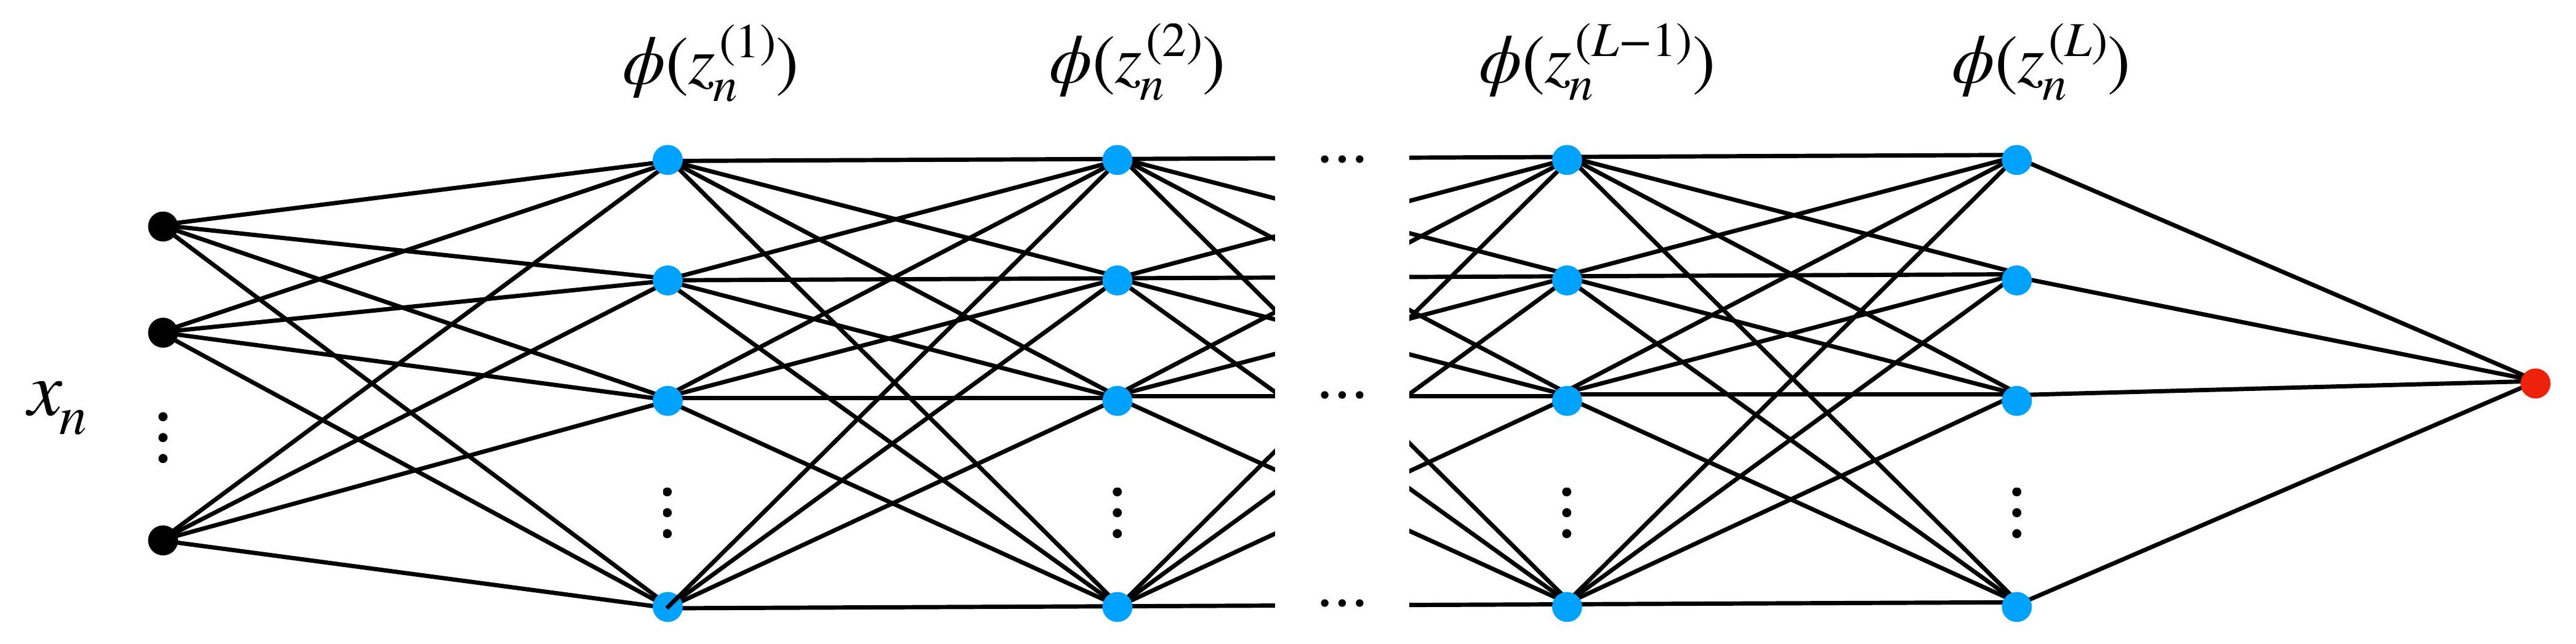
\includegraphics[max width=\textwidth, center]{2023_12_30_360102aa01a03e5a4270g-26}

\section*{Batch Normalization}
Consider a batch $B=\left(x_{1}, \cdots, x_{M}\right)$ and denote by $z_{n}^{(l)}$ the layer's pre-activation input corresponding to the observation $x_{n}$

\begin{center}
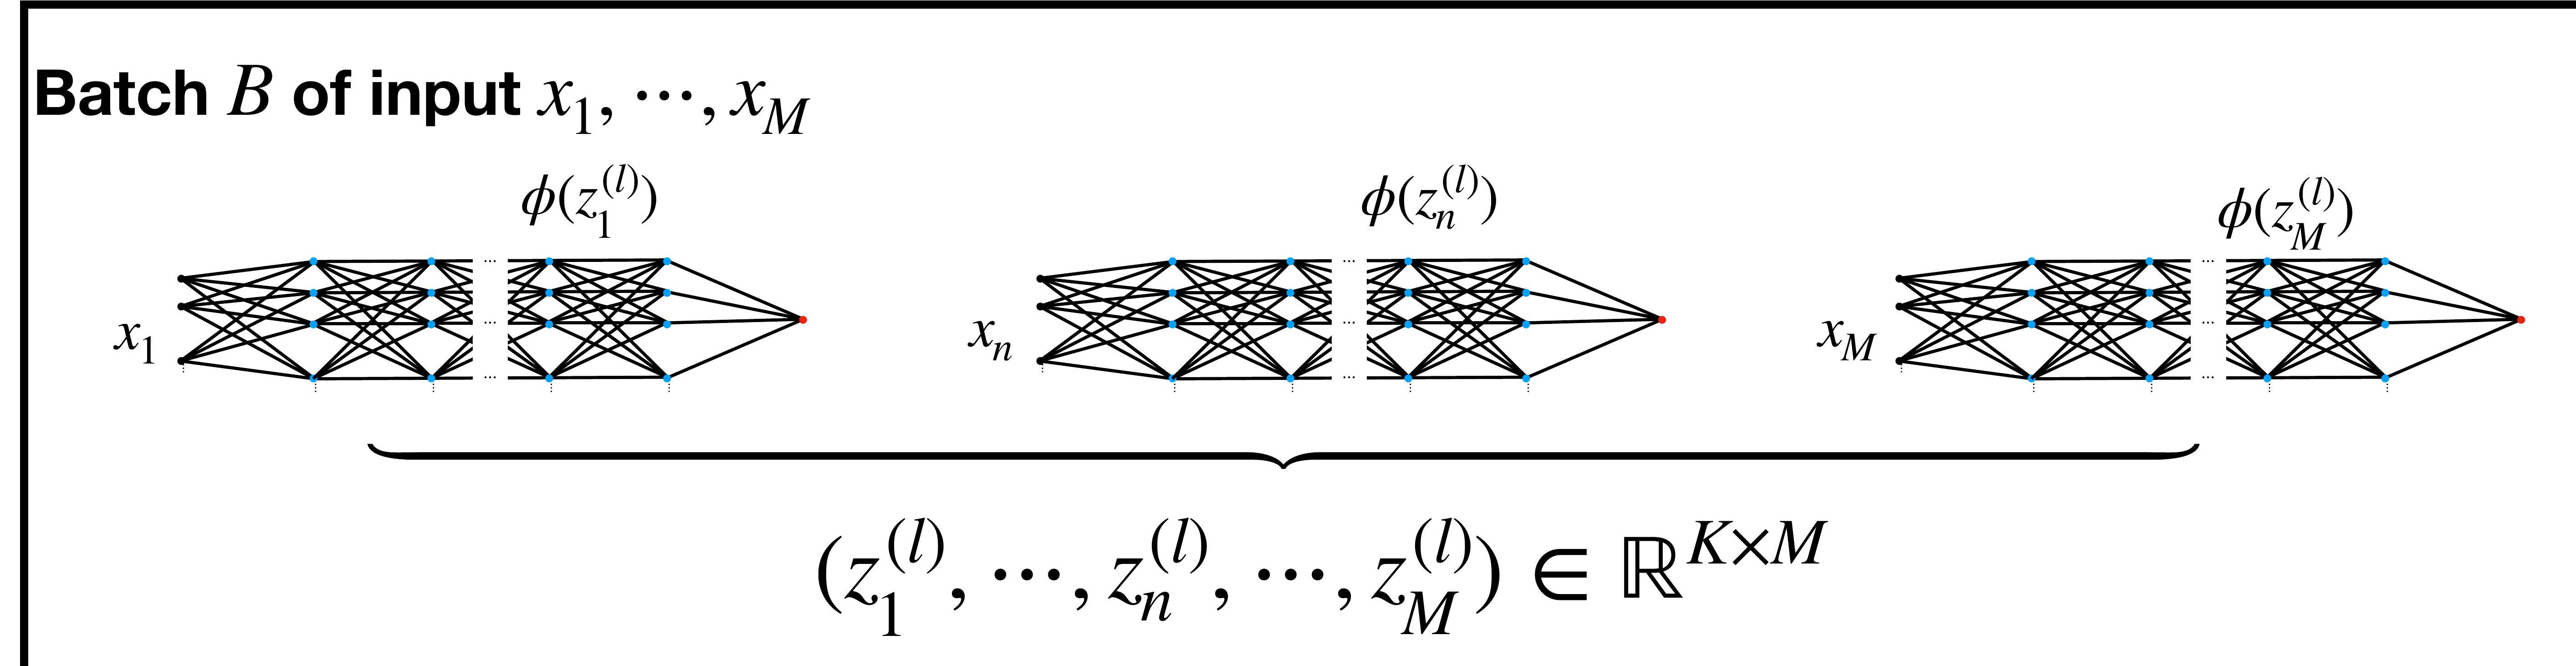
\includegraphics[max width=\textwidth]{2023_12_30_360102aa01a03e5a4270g-27}
\end{center}

\section*{Batch Normalization}
Consider a batch $B=\left(x_{1}, \cdots, x_{M}\right)$ and denote by $z_{n}^{(l)}$ the layer's pre-activation input corresponding to the observation $x_{n}$

Step 1: Normalize each layer's input using its mean and its variance over the batch:

$$
\bar{z}_{n}^{(l)}=\frac{z_{n}^{(l)}-\mu_{B}^{(l)}}{\sqrt{\left(\sigma_{B}^{(l)}\right)^{2}+\varepsilon}}
$$

Component-wise

where $\mu_{B}^{(l)}=\frac{1}{M} \sum_{n=1}^{M} z_{n}^{(l)}$ and $\left(\sigma_{B}^{(l)}\right)^{2}=\frac{1}{M} \sum_{n=1}^{M}\left(z_{n}^{(l)}-\mu_{B}^{(l)}\right)^{2}$, and $\varepsilon \in \mathbb{R}_{\geq 0}$ is a small value added for numerical stability

Step 2: Introduce learnable parameters $\gamma^{(l)}, \beta^{(l)} \in \mathbb{R}^{K}$ to be able to reverse the normalization if needed:

$$
\hat{z}_{n}^{(l)}=\gamma^{(l)} \odot \bar{z}_{n}^{(l)}+\beta^{(l)}
$$

\section*{Batch Normalization}
Scale-invariance: For $\varepsilon \approx 0$, the output is invariant to activation-wise affine scaling of $z_{n}^{(l)}$

$$
\mathrm{BN}\left(a \odot z_{n}^{(l)}+b\right)=\mathrm{BN}\left(z_{n}^{(l)}\right) \text { for } a \in \mathbb{R}_{>0}^{K} \text { and } b \in \mathbb{R}^{K}
$$

Thus, for example, there is no need to include a bias before BatchNorm.

Inference: The prediction for one sample should not depend on other samples

\begin{itemize}
  \item Estimate $\hat{\mu}^{(l)}=\mathbf{E}\left[\mu_{B}^{(l)}\right]$ and $\hat{\sigma}^{(l)}=\mathbf{E}\left[\sigma_{B}^{(l)}\right]$ during training, use these for inference
  \item Exponential moving averages are commonly used in practice
\end{itemize}

Implementation:

\begin{itemize}
  \item Requires sufficiently large batches to get good estimates of $\mu_{B}^{(l)}, \sigma_{B}^{(l)}$
  \item BatchNorm is applied a bit differently for non-fully-connected nets (see the pytorch docs for CNNs)
  \item In PyTorch, switch modes by using model.train() for training and model.eval() for inference
\end{itemize}

\section*{Batch Normalization - Results}
\begin{center}
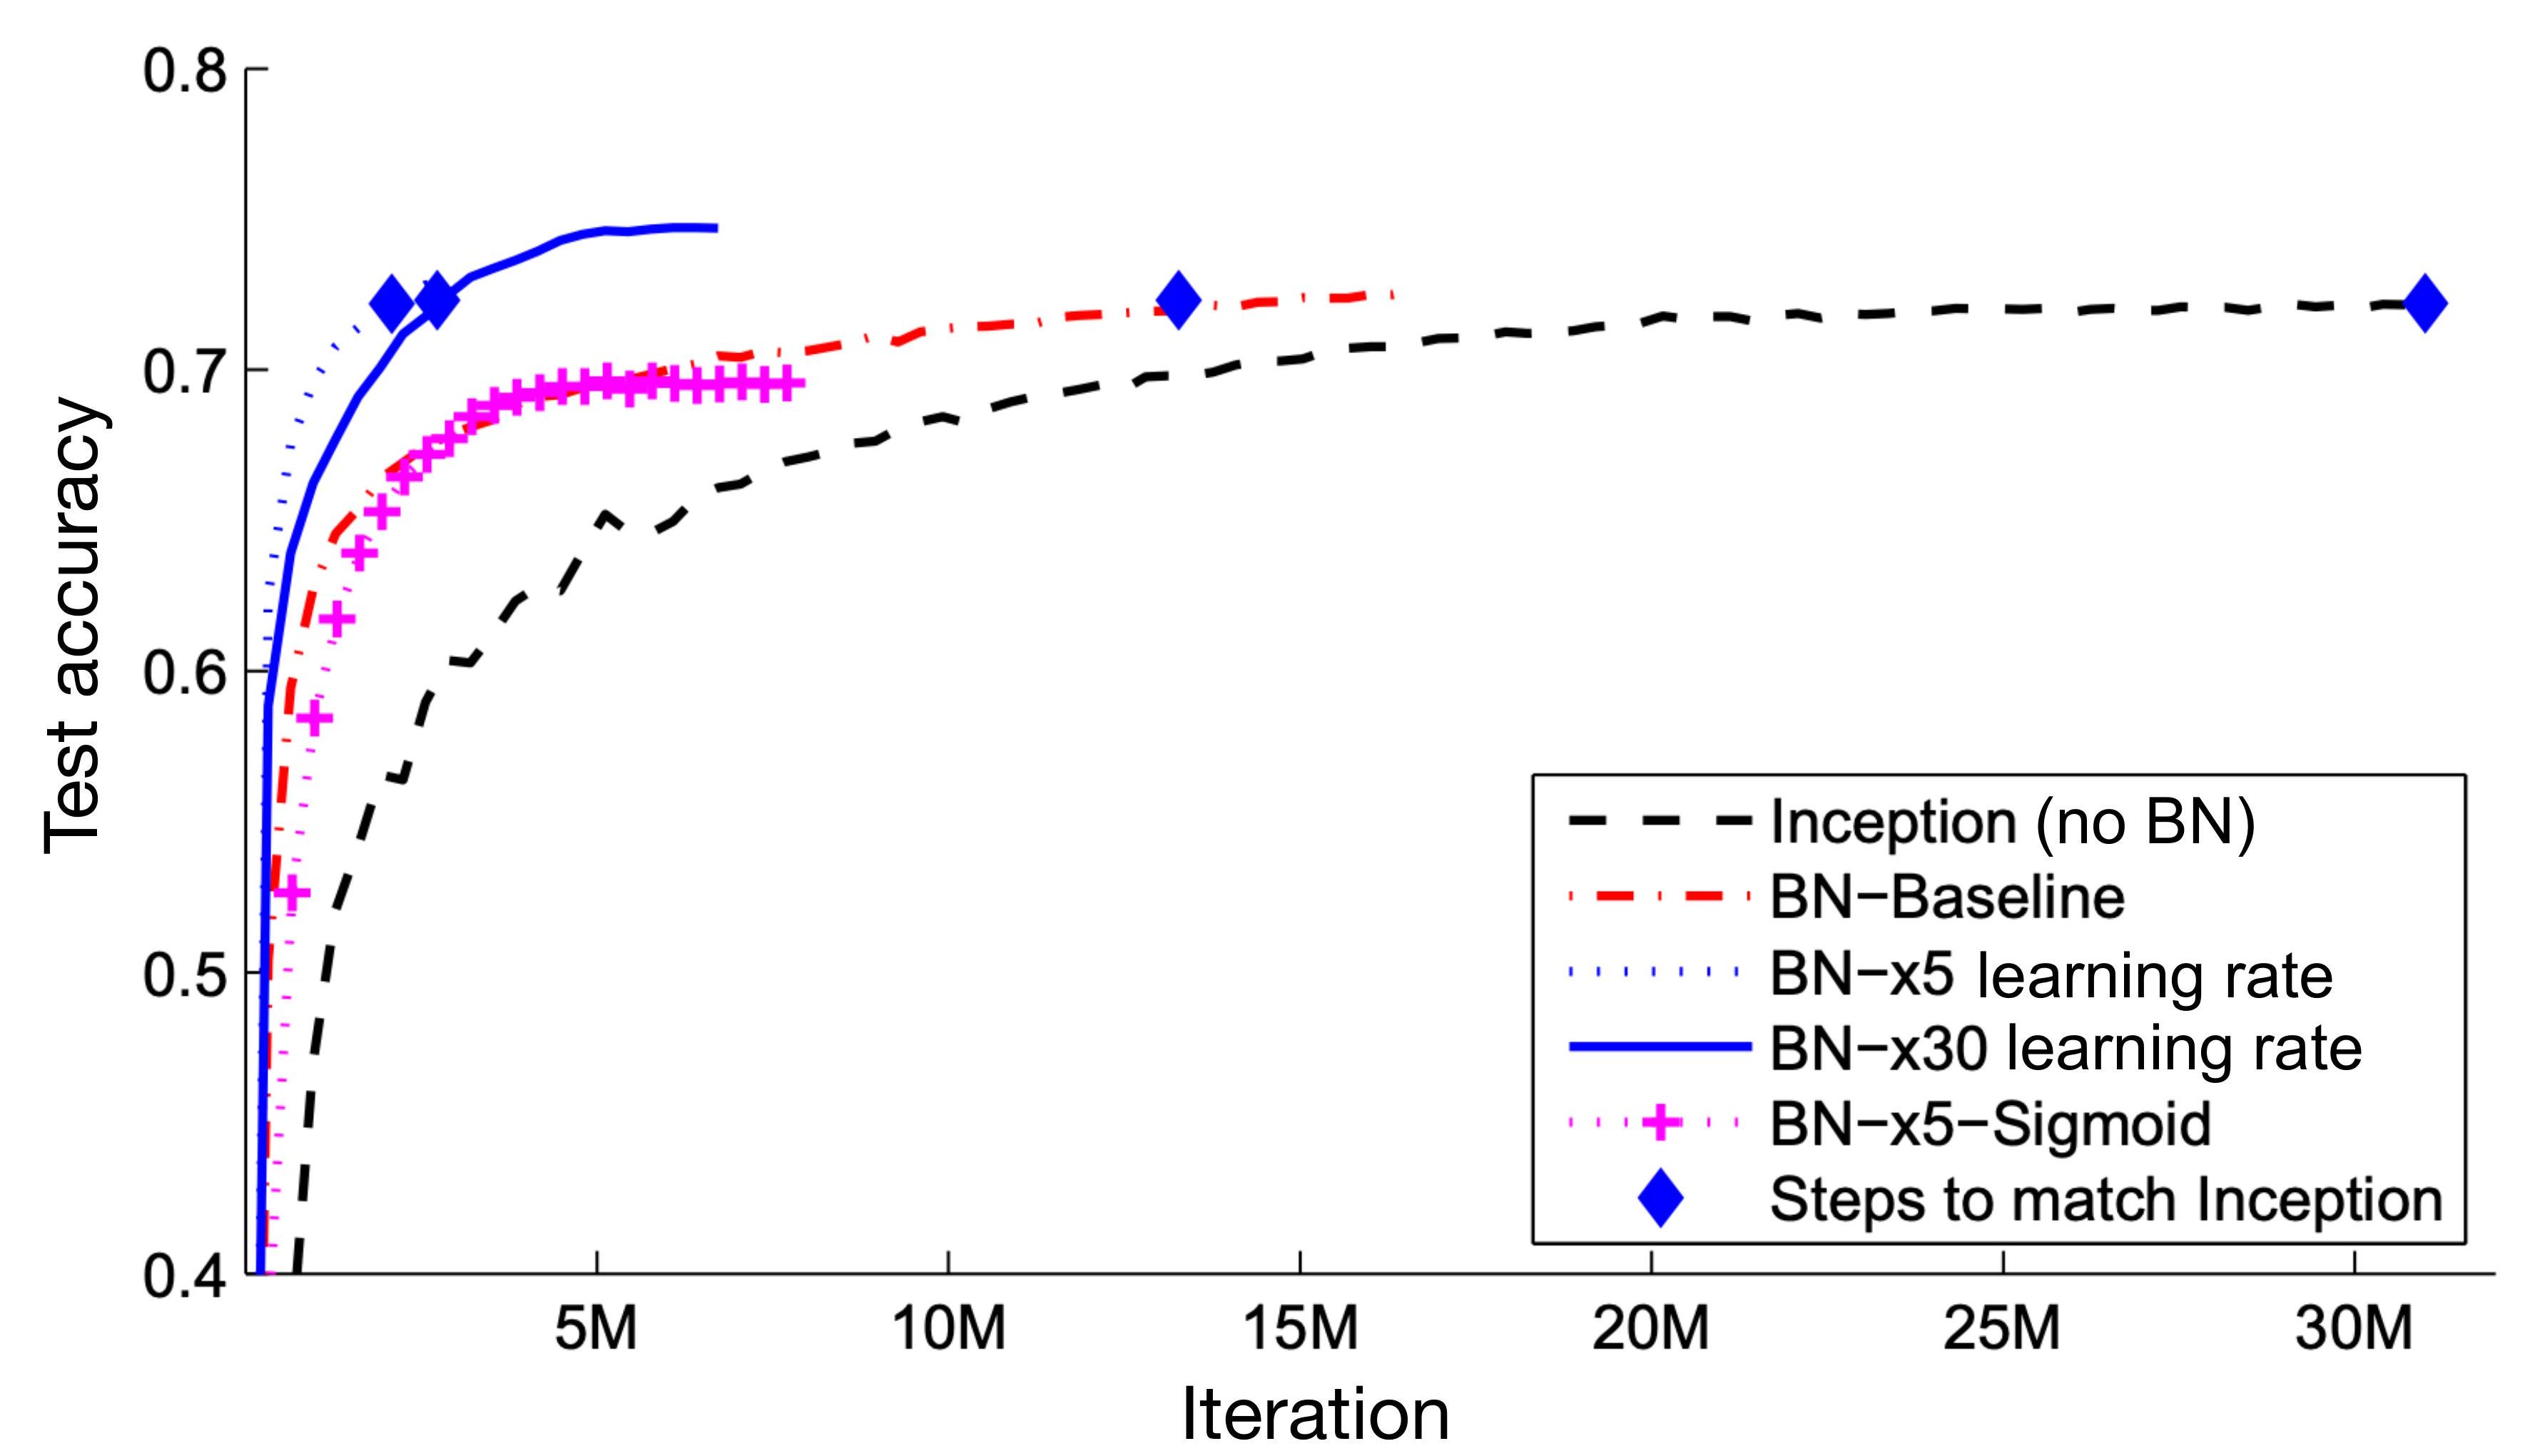
\includegraphics[max width=\textwidth]{2023_12_30_360102aa01a03e5a4270g-30}
\end{center}

Source: Batch Normalization: Accelerating Deep Network Training by Reducing Internal Covariate Shift (ICML 2015)

\begin{itemize}
  \item BatchNorm leads to much faster convergence
  \item BatchNorm allows to use much larger learning rates (up to $30 \times$ )
\end{itemize}

\section*{Layer Normalization}
Step 1: Normalize each layer's input using its mean and its variance over the features (instead of over the inputs):

$$
\bar{z}_{n}^{(l)}=\frac{z_{n}^{(l)}-\mu_{n}^{(l)} \cdot 1_{K}}{\sqrt{\left(\sigma_{n}^{(l)}\right)^{2}+\varepsilon}}
$$

where $\mu_{n}^{(l)}=\frac{1}{K} \sum_{k=1}^{K} z_{n}^{(l)}(k)$ and $\left(\sigma_{n}^{(l)}\right)^{2}=\frac{1}{K} \sum_{k=1}^{K}\left(z_{n}^{(l)}(k)-\mu_{n}^{(l)}\right)^{2}$, and $\varepsilon \in \mathbb{R}_{\geq 0}$

Step 2: Introduce learnable parameters $\gamma^{(l)}, \beta^{(l)} \in \mathbb{R}^{K}$ :

\section*{Remarks:}
$$
\hat{z}_{n}^{(l)}=\gamma^{(l)} \odot \bar{z}_{n}^{(l)}+\beta^{(l)}
$$

\begin{itemize}
  \item Normalize across features, independently for each observation
  \item Very common alternative, widely used for transformers and text data
  \item No batch dependency, use the same for training and inference
\end{itemize}

\section*{Normalization - conclusion}
Benefits of normalization layers:

\begin{itemize}
  \item Stabilizes activation magnitudes / reduces initialization impact
  \item Additional regularization effect from noisy $\mu_{B}^{(l)}, \sigma_{B}^{(l)}$ in batch norm
  \item Stabilizes and speeds up training, allows larger learning rates
\end{itemize}

Used in almost all modern deep learning architectures

\begin{itemize}
  \item Often inserted after every convolutional layer, before non-linearity
\end{itemize}

\section*{Recap}
\begin{itemize}
  \item Neural networks are trained with gradient-based methods such as SGD

  \item To compute the gradients, we use backpropagation, which involves the chain rule to efficiently calculate the gradients based on the network's intermediate outputs $z^{(l)}$ and $\delta^{(l)}$

  \item Proper parameter initialization should avoid exploding and vanishing gradients by carefully controlling the layerwise variance

  \item Batch and Layer normalization dynamically stabilize the training process, allowing for faster convergence and the use of larger learning rates

\end{itemize}

\end{document}